\documentclass[11pt]{book}
%\usepackage{proceed2e}
\usepackage{naacl}
\usepackage[hyphens]{url}


%%%% Fill out all these macros
\newcommand{\thesisTitle}{Persian Fake News Detection using Stance Classification}
\newcommand{\authorName}{Mahsa Ghaderan}
\newcommand{\advisor}{Main Guardian}
\newcommand{\advisorTitle}{Dr. Sauleh Eetemadi} % assistant, associate prof?
\newcommand{\advisorDepartment}{Computer Science and Engineering}


\newcommand{\readingCommitteeOne}{Dr. Behrouz Minaei-Bidgoli}			
\newcommand{\graduationYear}{2021}


%\usepackage{} -- add any other packages you want
\usepackage{amsfonts}
\usepackage{multirow,tabularx}
\usepackage{listings}
\usepackage{makecell}
\usepackage[linesnumbered]{algorithm2e}
\usepackage{amssymb}
\usepackage{graphicx}
\usepackage{amsmath}
\usepackage{float}
\usepackage{fullpage}
\usepackage{mathrsfs}
\usepackage{subcaption}
\usepackage{hyperref}% http://ctan.org/pkg/hyperref
\hypersetup{%
  %colorlinks = true,
  linkcolor  = black
}
\usepackage{mdwlist}
\usepackage{xspace}
\usepackage{setspace}
\usepackage{times} % Set the typeface to Times Roman
\usepackage[scaled]{helvet} % ss
\usepackage{courier} % tt
\usepackage[T1]{fontenc}


%\usepackage[showframe=true]{geometry}
\usepackage{changepage}
\usepackage[labelfont=bf]{caption} % boldface caption title for floats
\usepackage[square]{natbib}
\usepackage{enumitem}
\usepackage{natbib}
\usepackage{array,multirow}

\usepackage{booktabs}
\usepackage{bbm}
\usepackage{soul}
\usepackage{relsize}
\usepackage{eso-pic}
\usepackage{xspace}
\usepackage{epsfig}
\usepackage{graphicx}
\usepackage{amsmath}
\usepackage{amssymb}
\usepackage{float}
\usepackage{multirow}
\usepackage{rotating}
\usepackage{balance}
\usepackage{wrapfig}
\usepackage{enumerate}
\usepackage{caption}
\usepackage{framed}
\usepackage{enumitem}
\usepackage{multirow}
\usepackage{graphicx}
\usepackage{color}
%\usepackage{tkz-graph}
\usepackage{caption}
\usepackage{subcaption}
\usepackage{mathtools}
\usepackage{pifont}
\usepackage{scrextend}
\usepackage{sidecap}
\usepackage{graphicx}
\usepackage{enumitem}

\usepackage{eqexpl}
\usepackage{comment}
\usepackage{amsmath}
\begin{document}

%% Replace all of the orange portions with your personal info

\begin{titlepage}
\begin{center}
\vspace*{\fill}
\singlespace
\thispagestyle{empty}
{\LARGE { \thesisTitle \\} %self-explanatory
\doublespacing
\vspace*{\baselineskip}
{\large \authorName }\\ %self-explanatory
\vspace*{1.5\baselineskip}
\large A Thesis
\\ submitted in partial fulfillment of the\\
requirements for the degree of\\
% \vspace*{\baselineskip}
‌Bachelor\\
\vspace{1.5\baselineskip}
% \begin{figure}[h]
%     \centering
%     
\includegraphics[width=3cm]{iust.jpeg}
% \end{figure}

Iran University of Science and Technology
\\ \graduationYear}\\ % add year in YYYY format (e.g. 2020)
\vspace{1.5\baselineskip}

%add reading committee (just the reading committee, not the supervisory committee):
\large \textit{Reading Committee:} \\

\ifdefined\secondAdvisor 
    \advisor, Co-Chair \\
    \secondAdvisor, Co-Chair \\
\else
    \advisor, Chair
\fi

\readingCommitteeOne \\

\ifdefined\readingCommitteeTwo
    \readingCommitteeTwo \\
\fi
    

\vspace{2\baselineskip}
  Program Authorized to Offer Degree: \\
Computer Engineering
  
% \newcommand{\advisor}{Main Guardian}
% % if you have two advisors, uncomment these two
% \newcommand{\firstAdvisor}{Parent One}
% \newcommand{\secondAdvisor}{Parent Two}
% \newcommand{\readingCommitteeOne}{First Reader}
% \newcommand{\readingCommitteeTwo}{Second Reader}

  
  
%%% Insert year and name:
  \vspace*{\fill}
  \clearpage
  \thispagestyle{empty}
  \singlespace{
  \copyright~Copyright \graduationYear \\ %add year in YYYY format (e.g. 2020)
  \vspace*{\baselineskip}
  \authorName} %self-explanatory
\end{center}
\end{titlepage}


\doublespacing

%% Replace all of the orange portions with your personal info

\thispagestyle{empty}
\begin{centering}
\vspace{1in}
Iran University of Science and Technology \\
\vspace*{1.\baselineskip}
{\bf Abstract}\\
\vspace*{1\baselineskip}

{\thesisTitle}\\ %self-explanatory
\vspace*{1.\baselineskip}
{\authorName} \\ %self-explanatory
\vspace*{1.\baselineskip}


\ifdefined\secondAdvisor
    Co-chairs
    \else
    Chair
\fi
of the Supervisory Committee:\\ %change to co-chair if co-advised 
\advisorTitle~\advisor\\ \vspace{-.5em} \advisorDepartment \\
\ifdefined\secondAdvisor
    \secondAdvisorTitle~\secondAdvisor\\\vspace{-.5em}\secondAdvisorDepartment \\
\fi
\end{centering}
\vspace*{\baselineskip}
These days increase in unauthenticated internet sources has led to spreading fake news vastly. Failure to detect misinformation promptly can have significantly irreparable damages on the walk of life. Recent researches have improved stance classification as a primitive step to detect fake news in English. Moreover, they have less focus on recognizing fake news. In this work, we have developed a deep learning model based on ParsBERT to improve the accuracy of the Persian stance classification. We over-sampled the available imbalanced dataset in Persian to compensate lack of data in such a low-resource language. Then, we implemented a model to detect fake news in Persian by using our best stance classifier and other manually extracted features. Consequently, we achieved an accuracy of 85\% for stance classification and 99\% for fake news detection on the employed dataset.

\bigbreak
\vspace*{3cm}
\bigbreak
Keywords: Machine Learning, Deep Learning, Natural Language Processing, BERT, Oversampling, Stance Classification, Fake News Detection

\chapter*{Acknowledgements}
%% self explanatory:

I want to give my warmest thanks to my supervisor, professor Sauleh Etemadi, Who made this project possible. He fully supports me and guides me. He also led me in each stage of writing and doing this report.  

Specially thanks to my mother, father, and my sister, who support me every single day of my life. They were motivating me in this way.

I am also thankful for my teammates and the friends Mr. Majid Zarharan, Mr. Mehdi Moghadami, Mr. Armin Gholami, and Miss Zahra Hosseini. They helped me to improve this project and giving me valuable advice. 

Finally, Thank God for letting me through all these hard days and give me such power to finish this work. I keep trusting you for my future. 
%% Replace all of the orange portions with your personal info

\clearpage

% if you need an extra blank page to make the dedications start on an odd number, then un-comment the following:
%%\clearpage\thispagestyle{empty}\mbox{}\clearpage 

\begin{center}
{\LARGE \textbf{DEDICATION}}
\hspace{0pt}
\vfill
{To {\color{orange}????}} %add whomever you want here
\vfill
\hspace{0pt}
\end{center}



\tableofcontents{}
\listoffigures
\listoftables
\clearpage


% \chapter {Literature Review}
% The major purpose of reviewing the literature is to determine what has already been done that relates to your topic. 
This section basically supports the background section by providing evidence for the proposed hypothesis.
describe all the studies that you have mentioned in the background section. 

present a more focused survey of the specific studies that are associated with the precise objective of your study.

learn more about the previous research published on the topic, and this eventually translates into literature review when you write your research paper.


{\color{orange}(book,chptr9,AlgorithmsCreate and PreventFakeNews)}
A research team 7 based at Canada’s Waterloo University broke down the fully
automated fact-checking process into four steps:
1. Retrieve documents relevant to the claim in question.
2. Determine the “stance” of each document, meaning
whether it supports, rejects, or is ambivalent/unrelated
to the claim.
3. Assign a credibility score to each document based on its
source.
4. Assign a truthfulness score to the claim by combining the
document stances weighted by the document credibility
scores (and highlight relevant facts/context from the
documents).

The first step can be a tricky one, because it is more open-ended than the matching step conducted by Full Fact, Logically, and Squash: rather than searching through a specific database of fact-checks for a match to the claim, one needs to scour the Web for any documents that might have information related to the claim. Google’s use of BERT to analyze the text in user search queries is bringing us closer to this task, but many challenges still remain.

The third step is essentially what Google and Facebook already do—through Google’s use of PageRank and human evaluators and through Facebook’s NEQ scores, as you saw in Chapters 6 and 8. 

The fourth step is straightforward once the first three are complete, so the Waterloo team decided to focus on

the second step—stance detection—to see how well that could be automated. They used a data set of fifty thousand articles to train a deep learning classification algorithm that looks at the body of each article and the headline of the article and estimates whether the body agrees with the headline, disagrees with it, discusses it without taking a stance, or is unrelated to the headline. Their algorithm scored a very respectable ninety percent accuracy, which was considerably higher than previous attempts by other researchers. 

The main insight in their work was to start with Facebook’s massive pre-trained deep learning algorithm RoBERTa and then do additional focused training to fine-tune the algorithm for the specific task at hand. This general process of fine-tuning a massive pre-trained deep learning algorithm is called “transfer learning,” and it has been an extremely successful method in AI, so it is not at all surprising that this is the right way to go when it comes to stance detection—it just wasn’t possible before BERT and RoBERTa came out.




{\color{orange}(book,chptr9,AlgorithmsCreate and PreventFakeNews)}
The Allen Institute for Artificial Intelligence (which you briefly encountered in Chapter 2 for its Grover system for detecting GPT-2 type generated text) developed a free tool called SciFact 8 to help with fact-checking medical claims related to COVID-19. The user types an assertion, or chooses from a list of suggestions, such as “Higher viral loads of SARS-CoV-2 are associated with more severe symptoms,” and a list of medical research publications is returned, each with an estimated score of how strongly it supports or rejects the assertion—similar to the Waterloo team’s stance detection—and a few potentially relevant excerpts from each publication are provided.

When I tried this higher viral load assertion, seven articles were returned, four supporting and three refuting—and while not all of them seemed relevant or accurately labeled, the results were enough to show that there is not a strong scientific consensus on this issue.

Their algorithm uses BERT to process text, and it was fine-tuned as follows. 

First, a modestly sized collection of medical publications was assembled and the citation sentences (i.e., sentences that include a citation to another research publication) were extracted. Next, human experts manually rewrote these sentences as medical assertions; they were allowed to use the text surrounding each citation sentence, but not the paper being cited. The human experts also created negated versions of these assertions, so that the algorithm would have examples of assertions refuted by the literature, not just ones supported by it. They then went through by hand and decided
whether each assertion is indeed supported by the article it cites, or refuted by it, or whether there is insufficient information to make this decision—and in the cases where it was labeled as supported or refuted, the experts highlighted the passages in the article’s abstract that provided the strongest basis for this label. 

Roughly speaking, this process is how they trained their BERT-based algorithm to do all three tasks involved: retrieve articles relevant
to a given assertion, estimate the stance of each article in relation to the assertion, and extract relevant passages from each article’s abstract. 
The researchers’ framework in principle applies to all kinds of medical and scientific assertions—not just COVID-related ones—but since training their algorithm involves careful manual work with the data, they decided to launch this tool initially in a limited setting and scope. The reader is cautioned, and the researchers readily admit, that this tool is largely intended to show what is possible and what challenges remain, rather than to be blindly trusted. They tested a few dozen COVID-19 assertions and found the algorithm returned relevant papers and correctly identified their stance about two-thirds of the time. While this tool should not replace finding and reading papers manually, it might still help with a quick first-pass assessment of medical claims.


\chapter {Introduction}
These days, fake news and false information have been vastly flooding the Internet by numerous not verified news agencies with aims ranging from affecting individual people’s beliefs and decisions to influencing major events such as political elections (\cite{memory_network}). As days go by, the importance of detecting stance automatically is appealing more attention. Insofar as it has been suggested that automatic stance detection is the first step towards assisting human fact checkers to detect inaccurate claims \cite{UCLMR}.


%these notions by Claire Wardle from First Draft, 2 misinformation is “unintentional mistakes such as inaccurate photo captions, dates, statistics, translations, or when satire is taken seriously.”, and disinformation is “fabricated or deliberately manipulated audio/visual context, and also intentionally created conspiracy theories or rumours.”.\cite{stace_survey}

The purpose of automatic stance detection is to find the type of a relation between specified sentences against a given text by utilizing machines. So it is possible to evaluate what is the orientation of a news source towards a particular issue \cite{UCLMR}. The selected sentence could be a claim, a news item, an idea, a social network post, or any other source. Also, the text could be retrieved from news agencies, weblogs, posts that are shared on social media, and any other available text. Choosing the source and context of sentences and texts depends on the goal of the defined task. Four considered labels are \textit{Agree}, \textit{Disagreed}, \textit{Discussed}, and \textit{Not Enough Information}. 

Gathering a sufficient amount of data is a vital step to achieve reliable predictor model. Both number of records in the dataset and the quality of each sample have a significant effect on prediction accuracy. \cite{takestancefake}) gathered fifty thousand articles-headline pairs for their dataset, and achieved a respectable ninety percent accuracy, which was considerably higher than previous attempts by other researchers (\cite{book_fake}). Though, in some contexts, there isn't enough available data. Here is where transfer learning methods play a vital role and compensate lack of data. We pre-trained a model on a large text corpus in a general context and then fine-tune the model on task-specified data. \cite{takestancefake} used RoBERTa model which is pre-trained on Facebook data. Then fine-tune it on the specific task at hand.
Also, \cite{stance_robust} improved its accuracy by fine-tuning BERT model.

Researchers have suggested various methods for stance classification. One cluster of methods mainly focuses on deep learning approaches. The precision of models is improved by using word embeddings such as BERT, using recurrent neural networks such as LSTM, BiLSTM (\cite{stanceCI}), and utlizing attention-based network (\cite{stanceCI}). Besides, novel model architectures such as Memory Network (\cite{memory_network}), are currently proposed.

One possible way of evaluating the veracity of a given claim is detecting the stance of that claim against available trusted sources. Stance detection task traditionally were used in political and ideological debates fields \citep{stance_robust}. The idea of using Stance Detection techniques to analyze news items correctness has become caught researchers attention since 2016. Consistency of a sentence through sources can be retrieved by stance detection methods. Consequently, stance detection can be considered as a subtask of fake news detection (\cite{book_datafake}), and It is easier to judge a claim by its stance against other sources. So estimating the stance of a particular claim against available documents can be the first step in detecting fake news. 


\chapter {Literature Review}
A brief description of adopted algorithms which are used in this project are available in this chapter. Algorithms are classified as \textit{\hyperref[lr:tokenization]{Tokenization}}, \textit{\hyperref[lr:wordrep]{Words Representaion}}, 
\textit{\hyperref[lr:ml]{Machine Learning}},  
\textit{\hyperref[lr:oversampling]{Oversampling}},  
\textit{\hyperref[lr:lm]{Language Models}}, and  
\textit{\hyperref[lr:evalmetrics]{Evaluation Metrics}}. 
\section{Tokenization}
\label{lr:tokenization}
It is vital in the tokenizing step to break the corpus into correct words. Tokenizers limit the number of words to reduce computational costs, so it may happen that tokenizers generate meaningless words if the number of accepted words has not been set sufficiently. Also, sometimes tokenizers have not seen words before, and omit them while tokenizing the corpus. According to stated reasons, it is important to choose a tokenizer carefully.

\subsection{NLTK}
NLTK\footnote{nltk.org} (Natural Language ToolKit)) is a python platform to work easier with human language data. This tool kit supports more than 50 datasets and supports numerous languages including Persian. \ac{NLTK} supports various tokenizer methods. Its basic algorithm tokenize words depends on white spaces.

\subsection{Hazm}
Hazm\footnote{\label{fn:hazm}sobhe.ir} is a python library Persian language processing tool kit. It has variety of functions such as word and sentence tokenizer, word lemmatizer, POS tagger, Shallow, and Dependency parser. \textit{Hazm} tokenizer is \textit{\ac{NLTK}} compatible\footref{fn:hazm}.
		
\subsection{Stanza}
Stanford NLP group has released Stanza tool\footnote{stanfordnlp.github.io/stanza}. Stanza is also another advantageous NLP tools package and can diagnose multi-word tokens. At first, it splits raw input text into sentences, then performs sentences segmentation. It is efficient for linguistic analysis and supports more than 70 human languages and releases new versions constantly.
	
\subsection{WordPiece}
WordPiece tokenizer used by \ac{BERT} (\cite{bert}) machine learning model. \ac{BERT} is a transformer-based machine-learning model which is currently used in various natural language processing tasks. WordPiece algorithm starts learning tokenization with a list of available characters in the text. Then it expands its word list by merging the most repeated group of characters. This procedure continues until hitting the considered number of words limit. 

\section{Word Representation}
\label{lr:wordrep}
To represent a corpus, each token should be converted to a number or vector. Good representation carries semantic of each word or n-grams, sequential words contents, and is as brief as possible. Three baseline Bag-of-word (\cite{bow}), \ac{TFIDF} (\cite{tfidf}), and \ac{W2V} (\cite{word2vec}) algorithms are used in this project. In	 this section, these algorithms are described briefly.
\subsection{Bag of Word}
Bag-of-Words (\cite{bow}) model, is a way to represent texts. \ac{BoW} keeps words frequency and dismisses word's orders and context. Dimension of text representation is equal to the number of specified words plus one for words that don't exist in \ac{BoW} dictionary. Each cell in output vector representation stands for a specific word and the value of that cell is equal to the repetition times of that word in the particular text. As an alternative, it is possible to choose n-gram instead of a single word as \ac{BoW} dictionary. This may improve \ac{BoW} model performance in order to keep longer expression semantic but on the other hand dimension of representation exceed vastly. One disadvantage of \ac{BoW} is it doesn't specify any relation between words with similar semantic meanings\footnote{en.wikipedia.org/Bag-of-words\_model}. 

\subsection{Term Frequency–Inverse Document Frequency}

Term Frequency–Inverse Document Frequency (\cite{tfidf}) is an algorithm to present the importance of each word in a corpus in a statistical way (\ac{TFIDF}). According to the repetition of a specific word in each document and inverse effect of the number documents that the word appears in, a float number will be assigned to each word in that corpus.  
\begin{itemize}
	\item \textbf{Trem Frequency (TF):} This item represents how many times a word is used in each document. \textit{TF} should be calculated for each document separately. \textit{TF} term calculate from equation \ref{eq:tf}
	\begin{equation}
	\label{eq:tf}
	\text{tf} \left(t,D\right) = \frac{f_{t,d}}{\Sigma_{t^{`} \in d } f_{t^{`}, d}}
	\end{equation}
	
	\item \textbf{Inverse Document Frequency (iDF):} This term presents how much information a word has. The less repetition of a word through documents, the more information it has. This term is calculated from equation \ref{idf}. 
	\begin{equation}
	\label{idf}
	\text{idf} \left( t,D\right) = \log \frac{N}{\left|\{d\in D, t \in d\}\right| }
	\end{equation}
\end{itemize}

\noindent
After calculating \textit{TF} and \textit{iDF}, \ac{TFIDF} value for each word calculates from equation \ref{tfidf}.
\begin{equation}
\label{tfidf}
\text{tf-idf}\left(t,d,D\right) =  \text{tf} \left( t,D\right) . \text{idf} \left( t,D\right)
\end{equation}


\subsection{Word2Vec}
Word2vec (\cite{word2vec}) is a neural network-based model which learns each word semantic and even it can recommend words with similar meaning to a specific word. \ac{W2V} represents each word with a vector instead of a number. After the training phase, each word vector serves numbers that are generally similar to words with similar meaning, and words with less correspondence have lower vector similarities. This vector is called word-embedding. It is necessary to have a large corpus in order to train a powerful model which can predict each word vector precisely. Multiple alternative algorithms for \ac{W2V} exist. For example, Fasttext is an extension of \ac{W2V} model which treats each word as concatenated n-grams\footnote{en.wikipedia.org/wiki/Word2vec}.  



\section{Machine Learning}
\label{lr:ml}
Machine learning algorithms aim to learn patterns on a corpus of data while training procedure, then predict classes of news articles test data by those patterns (\cite{book_fake}). Machine learning algorithms have powerful performance even in complex problems. In comparison to deep learning models, Machine learning algorithms learn patterns according to their fed manually extracted predictors, and we don't have any other choice rather than relying on those number of extracted predictors (\cite{book_fake}). So extracting useful features  is a critical step in machine learning. The more meaningful and suitable predictors they see for a task, the better patterns they can find during the training procedure. In this section, a brief overview of \textit{Gaussian Naive Bayes}, \textit{SVC}, \textit{LinearSVC}, \textit{Random Forest}, and \textit{Logistic Regression} is available
\subsection{Gaussian Naive Bayes}
The first machine learning algorithm used to classify stance is Gaussian Naive Bayes Classifier (\cite{GNbayes}). It is an alternative to machine learning Naive Bayes classifier that is inspired by Bayes Theorem\footnote{en.wikipedia.org/wiki/Naive\_Bayes\_classifier}:

\[ P\left(y | X\right) =   \frac{P(X|y).P(X)}{P(y)} \]
where:
\begin{eqexpl}[25mm]
	\item{$X$} List of predictors that are independent of each other.
	\item{$y$} Label of a class.
	\item{$P\left(X|y\right)$} Probability of class with label $y$ from given X predictors.
\end{eqexpl}
Naive Bayes Classifier algorithm estimates the probability of each class. Gaussian Naive Bayes means that predictors are continuous and follow Gaussian distribution:

\[p\left(x=\upsilon | C_{k}\right) = \frac{1}{\sqrt{2\pi\sigma_{k}^{2}}}e^{-\frac{\left(\epsilon-\mu_{k}\right)^{2}}{2\mu^{2}_{k}}}\]
\begin{eqexpl}[25mm]
	\item{$C_{k}$} Class k.
	\item{$\mu_{k}$} Mean of $x$ values associated with $C_{k}$
	\item{$\sigma^{2}_{k}$} Bessel corrected variance x values associated with $C_{k}$
\end{eqexpl}

\subsection{Support Vector Machines}
\label{SVM}
SVC stands for \ac{SVM} Classifier. Support Vector Machines (\cite{svc})  are a group of supervised machine learning models. One of their applications is the classification problem. \ac{SVM} algorithms map each sample to a space such that samples of a particular class locate as far as possible from other classes samples. In other words, \ac{SVM} is looking for an n-dimensional hyperplane which can separate classes as clearly as possible\footnote{wikipedia.org/Support-vector\_machine}.

Regularization parameter stands for strength of regularization. Kernel of \ac{SVM} specifies the type of separator that the \ac{SVM} algorithm uses to distinguish different classes. It is a basic form of the mathematical function that \ac{SVM} tunes during the training procedure. Kernels of SVC could vary from a simple polynomial such as \textit{linear} to more complex ones such as \textit{Radial basis function}, \textit{Sigmoid}, and \textit{Higher degree polynomial}. Furthermore, the wight of each class could be different from each other. \textit{Balanced} mode set different weight for each class during training to compensate imbalanced data. 


\subsection{LinearSVC}
LinearSVC is an alternative algorithm for SVC in large datasets. LinearSVC linearly separates samples. Depends on the dataset, it may work better than nonlinear SVC. This model is the same as SVC from the previous part, the only difference is its kernel is equal to linear hyperplane polynomial. 

\subsection{Random Forest}
Random Forest (\cite{randomforest}) is a machine learning algorithm to deal with complex classification problems. It constructs of many decision trees. The point is that it is more robust than decision threes. Besides Random Forest classifier doesn't need parameter tuning. Each decision three has its own prediction and the final prediction of the model is calculated bt majority voting of each tree output. 

\subsection{Logistic Regression}
Logistic Regression is a machine learning classification algorithm. Its functionality is mainly for Binary Classification. In multi-class datasets, logistic regression classifies one class vs rest. This algorithm uses Sigmoid function as its cost function and its prediction is based on probabilities. 

Logistic Regression has a number of parameters can be tuned due to the specified task. Penalization and regularization parameter could be \textit{l1} (Equation \ref{eq:logil}), \textit{l2} (Equation \ref{eq:logill}), or \textit{elasticnet} (Equation \ref{eq:logisel}). If $\; \rho \;$ parameter equals to 0.5 in Elastic-Net Penalization, means $\;l1\;$ and $\;l2\;$ have the same powers. 
\begin{itemize}
	
	\item $l1$
	\begin{equation}
	\label{eq:logil}
	min_{\omega,c} \; \frac{1}{2}\omega^{T}\omega + C \Sigma_{i=1}^{n} \log\left(\exp\left(-y_{i}\left(X^{T}_{i}\omega + c \right)\right) + 1 \right)
	\end{equation}
	\item $l2$
	\begin{equation}
	\label{eq:logill}
	min_{\omega,c} \; \left|\left|\omega\right|\right|_{1} + C \Sigma_{i=1}^{n} \log\left(\exp\left(-y_{i}\left(X^{T}_{i}\omega + c \right)\right) + 1 \right) 
	\end{equation}
	
	\item $elastic-net$
	\begin{equation}
	\label{eq:logisel}
	min_{\omega,c} \; \frac{1-\rho}{2}\omega^{T}\omega +\rho\left|\left|\omega\right|\right|_{1} + C \Sigma_{i=1}^{n} \log\left(\exp\left(-y_{i}\left(X^{T}_{i}\omega + c \right)\right) + 1 \right) 
	\end{equation}
	
\end{itemize}
where:
\begin{eqexpl}[25mm]
	\item{$\rho$} Controls $\; l1 \;$ strength (\textit{l1\_ration} parameter).
	\item{$y_{i}$} Takes value between -1, 1.
\end{eqexpl}
\bigbreak
Another parameter specifies optimizer algorithm could be Minimizing Finite Sums with the Stochastic Average Gradient (\ac{SAG}), \ac{SAGA} which is an alternative of \ac{SAG} that supports $l1$ optimizer,  Newton’s method which utilize quadratic approximation, or Limited-memory Broyden–Fletcher–Goldfarb–Shanno which is analog to Newton's method and Hessian matrix is approximated by updating gradient evaluation and it is more robust in larger datasets. Although, Limited-memory Broyden–Fletcher–Goldfarb–Shanno is slower than \textit{SAGA}\footnote{scikit-learn.org/stable/modules/linear\_model.html\#logistic-regression}.

\section{Oversampling}
\label{lr:oversampling}
A common way of dealing with an imbalanced dataset is automatically augmenting samples to achieve balanced class distribution (Oversampling) or even reduce the number of samples in the majority class (Undersampling). Undersampling is applicable on a large dataset. But in small datasets, it's not wise to ignore some samples. Oversampling methods suites for datasets that suffer from lack of data. It is important to notice that splitting test and train sets should be performed before resampling, and oversampling should be only applied on the train set. RandomOverSampler, SMOTE, SVMSMOTE, BorderlineSMOTE, and \ac{ADASYN} algorithms are described in the following sections.

\subsection{Random Oversampler} 
This method randomly peak samples from classes and re-sample them. Random Over Sampler is the most naive algorithm and its performance is same as increasing minority class loss weight. Another variant of this method is smoothed bootstrap oversampling. It is generally similar to Random Oversampler, but new samples don't exactly overlap original samples. They are adjacent to source samples. This variant can be implement by \textit{shrinking} parameter in \textit{RandomOverSampler} from \textit{imblearn} python library\footnote{imbalanced-learn.org/stable/references/generated/imblearn.over\_sampling.RandomOverSampler.html}. 
	
\subsection{SMOTE}
Synthetic Minority Over-sampling Technique (\cite{smothe}) is an oversampling method by generating new samples by interpolation. It's not important for smothe sampler that point is chosen to be resampled. 
	
\subsection{SVM-SMOTE } 
SVMSMOTE (\cite{svmsmothe}) is a variant of SMOTE oversampling method which uses SVM (Section \ref{SVM}) algorithm to choose resampling samples. One strength of this model is that it is effective for both vector data and sequence data (\cite{svmsmothe})\footnote{imbalanced-learn.org/stable/references/generated/imblearn.over\_sampling.SVMSMOTE.html}.
	
\subsection{BorderlineSMOTE} 
BorderlineSMOTE (\cite{borderlinesmothe}) is also another variant of SMOTE oversampler. Borderline samples are mainly chosen to get resample in this variant. \cite{borderlinesmothe} has achieved better accuracy than SMOTE.\footnote{imbalanced-learn.org/stable/references/generated/imblearn.over\_sampling.BorderlineSMOTE.html}
\subsection{Adaptive Synthetic Sampling} 
Adaptive Synthetic Sampling Approach for Imbalanced Learning (\ac{ADASYN}) (\cite{adasyn}) focuses on generating new samples adjacent to those samples wrongly classified by employing K-Nearest Neighbors classifier. These samples are considered as hard samples because it's not easy for models to predict them, as a result, \ac{ADASYN} increases the robustness of the desired dataset. This method performs better in comparison to Decision Tree and SMOTE algorithms (\cite{adasyn}).

\section{Language Representation Model}
\label{lr:lm}
Language representation models can represent a word embedding in context. Pretrained language models have significant improve on many natural language model tasks such as natural language inference task (\cite{bert}). \ac{BERT}, \ac{ParsBERT}, and \ac{ALBERT} models are described in short in the following sections.
\subsection{BERT}
One of most impressive and powerful deep learning language model for text processing, is \ac{BERT} which is stands for Bidirectional Encoder
Representations from Transformers (\cite{bert}) and developed by Google. And has received state of the art result due its previous researches (\cite{bert}). \cite{spotfake} improved its performance by make usage of the \ac{BERT} language model in fake news detection. \ac{BERT} base version contains 12 transformer blocks, containing 110 million parameters. There are also another variant of \ac{BERT} such as large including 24 transformer blocks and multilingual \ac{BERT}. \ac{BERT} models are trained of Wikipedia corpus. 

One application of \ac{BERT} is using first top layers of \ac{BERT} model as contextual word embedding (\cite{book_datafake}). This model suggests a vector that representing a word which best fit in the current context.  \ac{BERT} is a masked language model. It randomly masks some tokens and learn to predict masked tokens correctly. \ac{BERT} utilizes bidirectional transformer, it means that \ac{BERT} can inferred text both left to right and right to left.

\subsection{ParsBERT}
ParsBERT (\cite{parsbert}) pre-trained model for Persian language that can be used at the top of the model. \ac{ParsBERT} model is a monolingual transfromer language model based on Google's \ac{BERT} model \cite{bert} which is lighert than multilingual \ac{BERT}. Pretrained \ac{ParsBERT} model is available on HooshvareLab\footnote{\href{https://huggingface.co/HooshvareLab}{huggingface.co}}. \ac{ParsBERT} outperforms other language model variants on Persian.

\subsection{A Lite BERT}
A Lite BERT (\cite{albert}) model is a lighter variant of \ac{BERT} model. The large \ac{BERT} model has 9 times more parameters than \ac{ALBERT}. \ac{ALBERT} is released by Google's team in 2019. It separates input and hidden layers embedding. The input layer is context-independent while the hidden layer is context-dependent. Same as \ac{BERT}, \ac{ALBERT} uses masked language model but instead of NSP (Next Sentence Prediction) \ac{ALBERT} uses SOP (Sentence Order Prediction) which only looks for sentence coherence in contrast to SOP which looks for both coherence and the topic to identify the next sentence.

 

\section{Evaluation Metrics}
\label{lr:evalmetrics}
The accuracy score is calculated from \ref{eq:acc}. It is good to evaluate the ratio of correctly predicted samples. Though accuracy score is not reliable to evaluate model performance specially when dealing with an imbalanced dataset. In addition to correctly predicted samples, False model prediction has an impact on the final F1 score (\ref{eq:f1}).   
\begin{equation}
\label{eq:acc}
\text{Accuracy} = \frac{\text{TP} + \text{TN} }{\text{TP} + \text{FN} + \text{TN} + \text{FP}}
\end{equation}
where:
\begin{eqexpl}[25mm]
	\item{$\text{TP}$} True Positive
	\item{$\text{TN}$} True Negative
	\item{$\text{FP}$} False Positive 
	\item{$\text{FN}$} False Negative
\end{eqexpl}

\begin{equation}
\label{eq:f1}
\text{F1} = \frac{2 \times \text{precision} \times \text{recall} }{\text{precission} + \text{recall}}
\end{equation}
where: 
\begin{eqexpl}[25mm]
	\item{$\text{precission}$} $\; \text{precision} = \frac{\text{TP}}{\text{TP} + \text{FP}} \;$
	\item{$\text{recall}$} $\; \text{recall} = \frac{\text{TP}}{\text{TP} + \text{FN}} \;$ 
\end{eqexpl}


\chapter {Related Works}
\label{literature}
Many researchers have done to improve stance detection accuracy. Different ideas and architectures have been applied. In the following part, previous research and papers have been overviewed.  

In 2016 \cite{Augenstein2016StanceDW} started working on the challenging task without assuming neither target is clearly mentioned in the text nor training date is given for every target. Their dataset construct of tweets mostly containing politicians and popular issues. The paper mainly focuses on detecting a stance with respect to unseen targets. \cite{Augenstein2016StanceDW} used conditional LSTM encoding on Tweeter data. \cite{Augenstein2016StanceDW} inferred that using unconditional LSTM has the best performance for unseen targets. Their results are improved by using bidirectional encoding. Using LSTM-based models lead to better results than Majority class, SVM (\cite{svc}), and BoW (\cite{bow}) as baselines in this experiment.

\cite{UCLMR} has developed an end-to-end stance detection system including lexical and similarity-based features which is passed through a multi-layer perception model. UCLMR's\footnote{UCL Machine Reading} model claimed third place in FNC-1\footnote{First stage of a competition Fake News Challenge(FNC-1) is exploring how artificial intelligence technologies could be leveraged to combat fake news\footnote{fakenewschallenge.org}. Numerous researchers has interest in this field and many papers has published besides this challenge.}. The model architecture is illustrated in Figure \ref{fig:UCLMR-system}. Headline and body texts are tokenized by scikit-learn\footnote{\cite{sikit-learn}}. Furthermore, \cite{UCLMR} used both term frequency (TF) vector of headline and claim and cosine similarity between head and body, and $l$2-normalized TF-IDF vectors. Besides, stop words are excluded. \cite{UCLMR} achieved FNC-1 score of 75.20\% on the test data set.
\begin{figure}
	\centering
	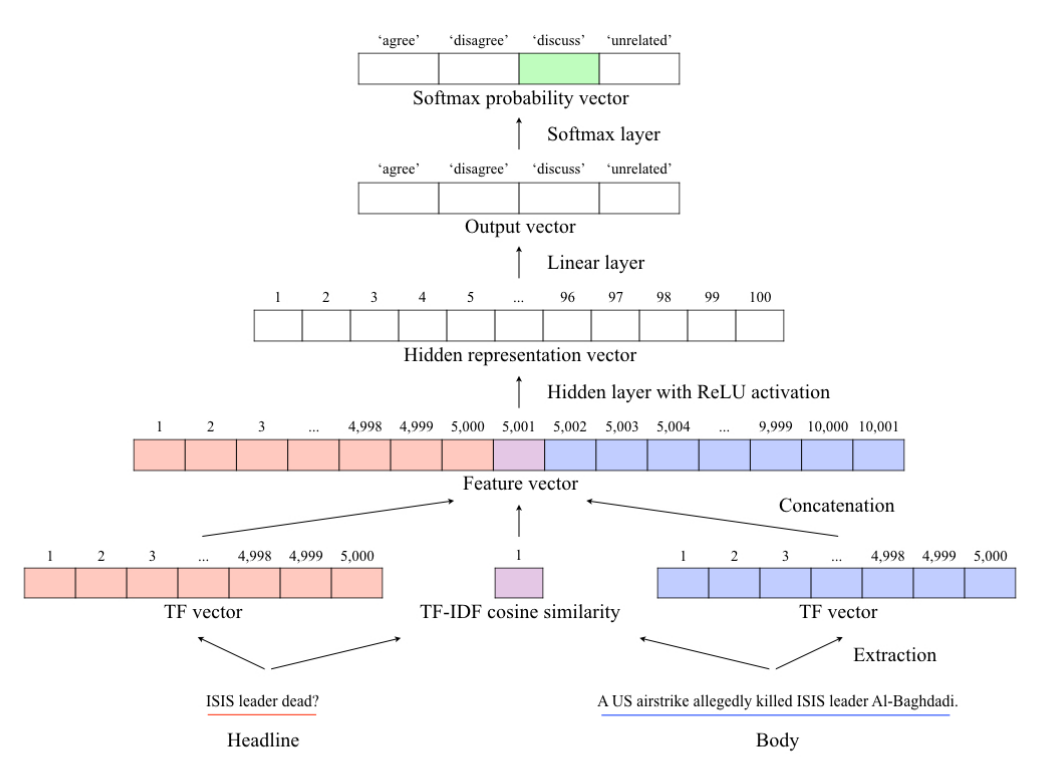
\includegraphics[scale=0.4]{statistics/stance/simple-baseline-FNC.png}
	\caption{Schematic diagram of UCLMR’s system.}
	\label{fig:UCLMR-system}
\end{figure}


\cite{Hierarchical-Attention-Network} have mainly focused on linguistic information such as polarity and argument of each document to represent a document. As shown in figure \ref{fig:hierarchical_att} document, sentiment, dependency, and argument representations are used in model architecture. \cite{Hierarchical-Attention-Network} concluded that every linguistic information with attention mechanism improves stance detection, And using linguistics features altogether outperform using them individually. More details are provided below.

\begin{itemize}
	\item \textbf{Document Representation}: \cite{Hierarchical-Attention-Network} used a LSTM model to represent each document.
	\item \textbf{Sentiment Representation}: As sentiment representation, an LSTM model is used to learn the representation of sentiment information. The sentimental word sequence of each document is extracted from sentiment lexicon. 
	\item \textbf{Dependency Representation}: This feature is used to capture inter-word relationships. Firstly, relations from the dependency parser are extracted. Then, representation of dependency sequence is learnt by using an LSTM layer.
	\item \textbf{Argument Representation}: The argument is considered as the author's stance. \cite{Hierarchical-Attention-Network} used a binary classification to detect the document's argument sentence. Then, it learned the sequence representation of word sequence in argument sentences by making use of LSTM layer.
\end{itemize}

In addition, it utilized a hierarchical attention network in order to weigh the importance of linguistic information, and learn the mutual attention between the document and linguistic information. \cite{Hierarchical-Attention-Network} mentioned that the Hyper Attention layer in Figure \ref{fig:hierarchical_att}, had a considerable influence on model performance. 

\begin{figure}
	\centering
	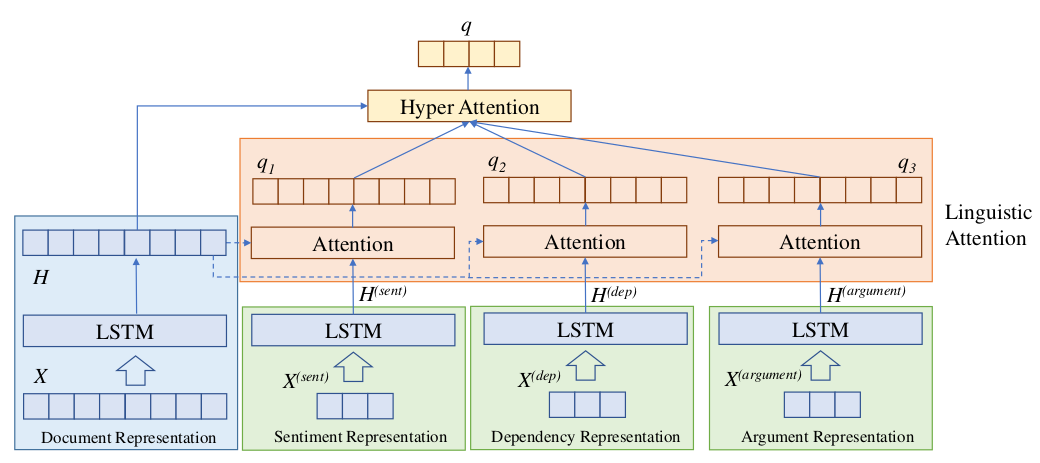
\includegraphics[scale=0.4]{statistics/stance/hierarchial-attention-network.png}
	\caption{Overview of \cite{Hierarchical-Attention-Network} model.}
	\label{fig:hierarchical_att}
\end{figure}

\cite{memory_network} present a novel end-to-end memory network in 2018 to predict stance and extract snippet of the prediction. The proposed model mainly focuses on relevant paragraphs. This model incorporates recurrent, convolutional neural networks and similarity matrixes. \cite{memory_network} mentioned that detecting \textit{Disagree} is the hardest label to predict. To overcome the imbalance issue, \cite{memory_network} select the same number from each class in each iteration. 
\begin{figure}
	\centering
	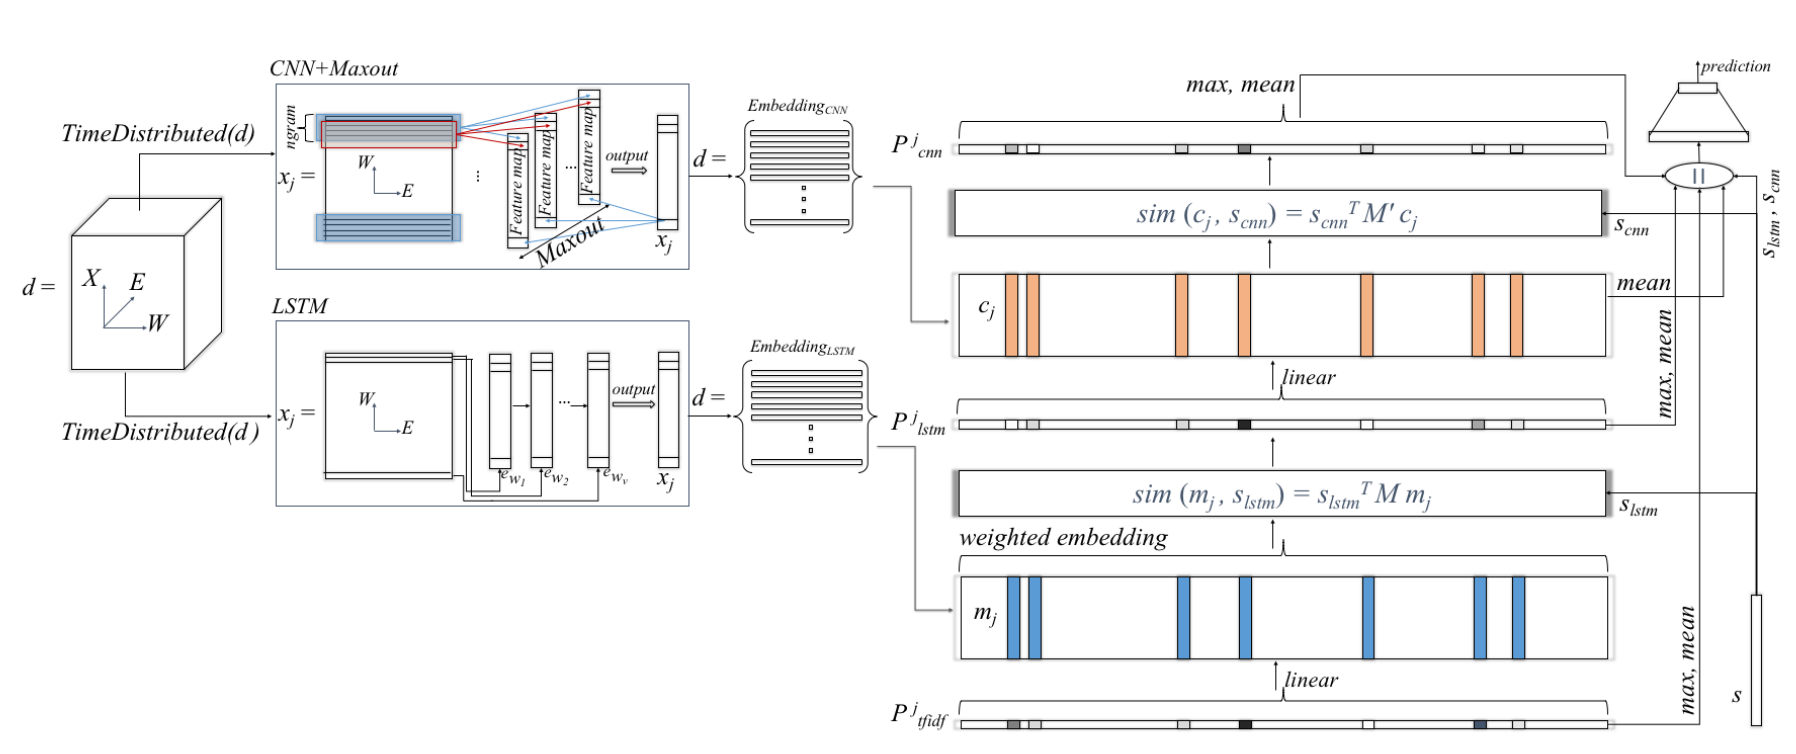
\includegraphics[scale=0.25]{statistics/stance/memoty_network.png}
	\caption{Architecture of Memory Network for the stance classification task.}
	\label{fig:mem_network}
\end{figure}

\cite{stance_robust} mainly focused on the robustness of a stance detection classifier. Trained models  on a single data set in a special domain, won't be robust enough on other domains. So they suggested using a multi-domain dataset or use multi-dataset learning methods to improve model generalization. The model architecture is constructed of fine-tuned BERT\cite{bert} and a single dense classifier at the top. \cite{stance_robust} used 5 fixed seed values during training and reported averaged results of trained models. \cite{stance_robust} concluded that MDL(multi-dataset learning) has a significant impact on increasing model robustness.



\chapter{Methodology}
\label{sec:exp}
We have used different ideas and methods in this project. In this chapter methods are explained in following 
\textit{\hyperref[mth:preproces]{Preprocessing}}, 
\textit{\hyperref[mth:wordrep]{Word Representation}}, 
\textit{\hyperref[mth:features]{Features}}, 
\textit{\hyperref[mth:ml]{Machine Learning}}, 
\textit{\hyperref[mth:balance]{Balancing}}, 
\textit{\hyperref[mth:dl]{Deep Learning}}, 
\textit{\hyperref[mth:a2c]{Article to Claim}}, and 
\textit{\hyperref[mth:fn]{Fake News Detection}} sections.

\section{Preprocessing}
\label{mth:preproces}
The first and mandatory preprocessing step is to tokenize words in the corpus in order to remove and detect special words. After tokenization, a list of punctuation and Persian stop-words are considered as \textit{denied} words and are removed from the corpus in this step. We chose stop-words carefully in a way not to lose refuting or supporting expressions in news context. Verbs carry valuable information to detect stance of an article. Nonverbal stop-word class is a better choice to remove low-value words in this task. Also English number characters will remove from the corpus before tokenizing. 

\section{Features}
\label{mth:features}
In machine learning algorithms, feature engineering can be considered the most important step because the desired model trains patterns only corresponding to predictors. Extracting sufficient predictors as compact as possible to having the best predicting accuracy and time-efficient	, requires numerous trials and errors. In the following part of this section, extracted features are explained in detail.

\subsection{Similarity}
The similarity score is offered by \cite{stance_persian}. This feature calculates how much a claim is similar to a headline or a news article, depends on the task. Three following sequence matching score is considered for this feature.

\begin{itemize}
	\item Ratio: Similarity score in float range 0,1. This parameters calculates from equation \ref{eq_ratio}
	\begin{equation}
		\label{eq_ratio}
		\text{ratio} = \frac{2.0 * M}{T}
	\end{equation}
	where:
	\begin{eqexpl}[25mm]
		\item{$T$}Number of elements in both sequences.
		\item{$M$}Number of matches.
	\end{eqexpl}
	\item Quick Ratio: This parameter estimates an upper bound on the Ratio.
	\item Real Quick Ratio: This parameter estimates an upper bound on the Ratio.
\end{itemize}

\subsection{Root Distance}
This feature is suggested by \cite{stance_persian}. Root Distance stands for the distance between the root of a headline and some collected hedge, refuting and reporting words. Firstly, a set of words considered as mentioned group are gathered, and then for each word distance is calculated.

\subsection{ImportantWords}
List of a controversial and challenging words in news gathered by \cite{stance_persian} and considered as \textit{important-words} in this project. This feature is a zero-based list with the length of important words, and each cell stands for one word in \textit{important-words}. The list carries the number of repetitions of desire words in a specific news article.
\subsection{Is Question}
Is-Question identifies whether a claim or headline of a news article ends with question marks or not. \cite{stance_persian} dataset contains a column dedicated to this feature.
\subsection{Has Two Parts}
Has-Two-Parts is if a claim is constructed of two separate parts. \cite{stance_persian} dataset contains a column dedicated to this feature.
\subsection{Polarity}  
The polarity of a text can be utilized in a variety of tasks. This feature presents how positive or negative a text is. Different algorithms are developed to predict the polarity of a text. In this project, \cite{persent} dataset is used to calculate each sample sentiment. \cite{persent} contains a dictionary of words with their sentiment score between -1 and 1. The more negative the word meaning, the lower its polarity point. For each word presents in each sample at most first 30 nonzero polarity value saves in a zero initialed vector with 30 lengths. As \cite{persent} contains only 1500 word polarity values, it can't cover all words in corpus and it has a far way to improve. 

In this project, an idea is applied to extend PerSent (\cite{persent}) polarity dataset is to use a language model. It is possible to predict similar words with a particular word and estimate their similarity score with a language model. Firstly, similar words that don't polarity score in PerSent with their similarity scores extract from a pre-trained language model. Then search each word in the PerSent dataset (\cite{persent}) and apply equation \ref{eq_polar} average through all similar words polarity scores, to estimate the desired word polarity score.

\begin{equation}
	\label{eq_polar}
	\text{polarity\_score}\left(w\right) = \frac{\Sigma_{w^{`} \in W} \text{Similatiry}\left(w^{`}, w\right) . \text{Polarity}\left(w^{`}\right)}{\Sigma_{w^{`} \in W} \text{Similatiry}\left(w^{`}, w\right)}
\end{equation}

where: 
\begin{eqexpl}[25mm]
	\item{$w$}Desire word $\notin$ PerSent datast.
	\item{$W$}Similar words, Predicted by the language model
	\item{$\text{Similarity}$}Similarity score for 2 words which is predicted by the language model.
	\item{$\text{polarity}$} Polaroty score which is estimated by \cite{persent} dataset.
\end{eqexpl}

\bigbreak
One alternative is to use a deep neural networks model to predict score polarity of a word whether word-level or sentence-level. But due to the lack of a Persian dataset in news context, it is not practical. Available datasets for sentiment analysis are mainly gathered from customer comments on special businesses. For instance \cite{polar_hotel} used 2 different datasets, first it translated English sentiment analysis corpus and second used comments on hotels. Besides, datasets containing polarity of comments of SnappFood\footnote{snappfood.ir} and DigiKala\footnote{digikala.ir} websites are available. One main problem with these datasets is the different use of language between user comments and news. Users mostly use everyday language on the other hand news agencies use formal language.



\section{Balancing}
\label{mth:balance}
Balancing methods is needed to compensate lack of data in classes except the majority class. Imbalance datasets make models to be biased on the majority class and there may be not enough samples in other classes for a model to learn that. This leads to having high accuracy score (Equation \ref{eq:acc}) while having low f1 score (Equation \ref{eq:f1}). There are several algorithms to deal with imbalanced datasets. It's not practical to rely on only one method and except to perform in the best way. Consequently, three different methods are applied on to the dataset in order to deal with this phenomenon. Methods of balancing a dataset which is used in this project are described in the following sections.  
	
\subsection{Extending dataset}
The simplest method is to gather data for classes except for the majority class. But unfortunately, it is not always practicable. Another way of extending a dataset is to use another existing dataset which has similar gathering logic and it is possible to map these two dataset classes. 

ParsFEVER (\cite{parsfever}) is a Persian dataset set based on FEVER (\cite{fever}) dataset is gathered for fact extraction and verification task. \cite{parsfever} claims are generated from Wikipedia\footnote{wikipedia.org} articles manually, then pieces of evidence for each claim are extracted from Wikipedia separately by distinct annotators. This dataset contains three \textit{Support}, \textit{Refute}, and \textit{Not Enough Info} classes. 
\begin{itemize}
	\item {\color{green!70!black}\textbf{Support:}} The article obviously proves the given claim. 
	\item {\color{red!60!black}\textbf{Refute:}} The article obviously disproves the given claim.
	\item {\color{gray}\textbf{Not Enough Info:}} There is not enough information in the article about the claim. 
\end{itemize}                

According to Figure \ref{fig:datacom} two \textit{Agree} and \textit{Disagree} class in \cite{stance_persian} dataset suffers from lack of samples. In this project, \textit{Supports} and \textit{Refutes} samples from \cite{parsfever} dataset are mapped to \textit{Agree} and \textit{Disagree} class of \cite{stance_persian} dataset respectively. 
But it is not possible to extend \textit{Discuss} or \textit{Unrelated} class by ParsFEVER, because they are both merged in \textit{Not Enough Info} class. As a result, two \textit{Agree} and \textit{Disagree} extended as much as possible with random selected samples from ParsFEVER dataset. Sample distribution is illustrated in figure \ref{fig:datab1}. Dataset is still imbalanced in one class for both Article-to-Claim (\ac{A2C}) and Headline-to-Claim (\ac{H2C}).


\subsection{Oversampling and Undersampling}
 Desired oversampling methods to deal with imbalanced dataset are RandomOverSampler, SMOTE, SVMSMOTE, BorderlineSMOTE, and \ac{ADASYN} which are described in section \ref{lr:oversampling}. 

\subsection{Tune model parameters}
 The last but not least important balancing method is to choose a robust learning algorithm for an imbalanced dataset, Choosing a weight of each class according to the ratio of samples of each class and choosing an optimizer and loss function that can overcome an imbalanced dataset.

\section{Machine Learning}
\label{mth:ml}
Figure \ref{fig:mlschm} illustrates a basic schematic of each machine learning models. Input of the model are samples in the dataset. After prepossessing, then predictors extracts from Feature Extractor module. The description of each predictor described in detail at section \ref{mth:features}. As the next step, before feeding data into classifier modules, balancing dataset is performed on dataset training set. Finally, samples classify in to one of four desired labels. 
\begin{figure}% 
	\centering
	{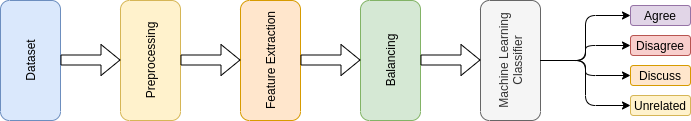
\includegraphics[width=14.5cm]{statistics/schema/ml.png} }
	\caption{Schematic of each machine learning model.}%
	\label{fig:mlschm}%
\end{figure}


\section{Deep Learning}
\label{mth:dl}
In the deep learning (\ac{DL}) approach, a combination of all predictors can be fed into the model and the model on its own will automatically learn which predictor is useful for the task. This property is the biggest advance of \ac{DL} in comparison to machine learning (\cite{book_datafake}). On the contrary, in machine learning (\ac{ML}), it was a critical step to design input predictors that the model can perform the best. And hours of trying different combination of predictors is needed (\cite{book_fake}). \cite{stance_robust} assessed that, In contrast, \ac{DL} models, \ac{ML}  models that are trained on a single dataset, usually generalize poorly to other domains.

The schematic of the \ac{DL} model is shown in figure \ref{fig:dlschm}. \ac{H2C} and \ac{A2C} models have the same schematic. Only the input shape of parameters varies in each model. In comparison to Figure \ref{fig:mlschm} Feature Extraction is omitted from the \ac{ML} model. Besides, The deep learning module constructs of pre-trained language model and a few Dense layers at its top. We evaluated \ac{BERT}, \ac{ParsBERT}, and \ac{ALBERT} language models against each other in this project (More description in section \ref{lr:lm}).
\begin{figure}% 
	\centering
	{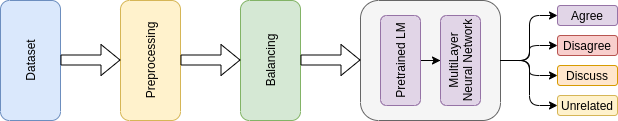
\includegraphics[width=14.5cm]{statistics/schema/dl.png} }
	\caption{Schematic of our deep learning model.}%
	\label{fig:dlschm}%
\end{figure}


\section{Article to Claim}
\label{mth:a2c}
Deep learning models perform far better on language inference tasks so they are better choices for \ac{A2C} stance classification. To calculate the stance of a claim toward the body of a news article, three different models based on a pre-trained Persian language model based on \ac{BERT}, \ac{ParsBERT}, and  \ac{ALBERT} (More description in section \ref{lr:lm}) are evaluated against each other. 

\section{Fake News Detection}
\label{mth:fn}
	\label{sec:fakenews}
Schematic of fake news pipeline is shown in figure \ref{fig:fnschm}. To detect a news article's veracity, \ac{H2C} and \ac{A2C} stance detection models, are considered as a black box. Four news articles are considered to evaluate the veracity of a claim. Firstly, the stance of a claim toward each headline of desired news articles and the body of the news article predict by stance classifier models. All predicted stance vectors are concatenated and along with some other features are fed into a multi-layer perception network in order to predict the veracity of the claim.

\begin{figure}% 
	\centering
	{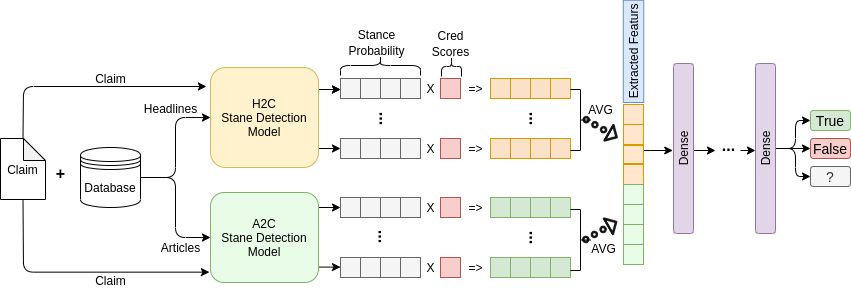
\includegraphics[width=14.5cm]{statistics/schema/fn.png} }
	\caption{Schematic of our fake news detection model.}%
	\label{fig:fnschm}%
\end{figure}

The credibility of news websites is one of the most important extracted features. The credibility can be calculated through the following steps (The credibility score of \ac{H2C} and \ac{A2C} is calculated similarly except using their related stance ground truth):

\begin{itemize}
	\item \textbf{Initialization}: The credibility score of all news websites that are existing in the \cite{stance_persian} dataset is set to zero at first. For the test set or predicting new samples, if the website doesn't exist in the data set, the credibility score is set to 0.1.


	\item \textbf{Quantification:}
	For each sample in the dataset, the credibility score changes according to Table \ref{tbl:cred}. $\rho$ value is calculated from equation \ref{eq:cred} if it is needed.
	\begin{table}[H]
		\centering
		\caption{Value of credibility according to GroundTruth and Veracity labels. }
		\setlength{\extrarowheight}{5pt}%
		\begin{tabular}{|l|l|l|}
			\hline
			GroundTruth & Veracity & Value \\
			\hline \hline
			Agree       & True     & $+1$    \\
			\hline
			Disagree    & False    & $+1$    \\
			\hline
			Agree       & False    & $-1$    \\
			\hline
			Disagree    & True     & $-1$    \\
			\hline
			Discuss     & True     & $+\rho$    \\
			\hline
			Discuss     & False    & $-\rho$   \\
			\hline
			Unrelated     & -   & No change   \\
			\hline
			-     & Discuss    & No change   \\
			\hline
		\end{tabular}
		\label{tbl:cred}
	\end{table}

	\begin{equation}
	\label{eq:cred}
	\rho = \frac{\text{P}(x,\text{Agree}) - \text{P}(x,\text{Disagree})}{\text{P}(x,\text{Agree}) + \text{P}(x,\text{Disagree})}\\
	\end{equation}

where: 
\begin{eqexpl}[25mm]
\item{$\text{P}(x,\text{Agree})$} Probability of Agree
\item{$\text{P}(x,\text{Disagree})$} Probability of Disagree 
\end{eqexpl}
	
	\item \textbf{Score Calculation:} The credibility score for each news website is calculated from equation \ref{eq:honesty}.
	\begin{equation}
	\label{eq:honesty}
	\text{H}(X) = \frac{\sum_{i=1}^{\text{k}_{X}} \text{credibility\,of\,}x_{i}}{\text{k}_{X}}
	\end{equation} 
	where:
	\begin{eqexpl}[25mm]
		\item{$\text{X}$} A news website
		\item{$\text{k}_{x}$} The number of news article in the dataset from x
		\item{$\text{credibility\,of\,}x_{i}$} Due to table \ref{tbl:cred}
	\end{eqexpl}

\end{itemize}


Also other features are extracted to detect fake news, such as :
\begin{itemize}
	\item One-hot encoding of the news website domain
	\item The ratio of samples that have been properly labeled as agree or disagree to the total sample of the news website (Correct ratio)
	\item The ratio of samples that have been wrongly labeled as agree or disagree to the total sample of the news website (Wrong ratio)
	\item The ratio of the total number of news website articles to the total number of articles in the data set.	
\end{itemize}





\chapter {Experiments}
\label{chapter:four}
In this section, experiment setups and the results of each experiment in each step are discussed. Besides, different ideas and algorithms which are described in section \ref{sec:exp} are evaluated. At first, machine-learning-based experiments are presented. As machine learning feature engineering, requires multiple experiments to find best working predictors, there are many trials and errors for a variety of algorithms and ideas. Then, Deep learning models are compared to machine learning models. Finally, the FakeNews model is evaluated depends on best stance detection models.

The headline of news is a summary of its body content and most of the time, it carries valuable data. So, we focused on detecting the news headlines stance towards claim(H2C), as well as the news articles stance towards a claim(B2C). According to the lower amount of text in the news headline, most of the experiments are firstly applied to H2C. Then, better approaches are applied to A2C.  


\section{Dataset}
\label{sec:dataset}
The first Persian stance detection dataset (\cite{stance_persian})  is used in this project. \cite{stance_persian} dataset can be used in stance detection, summarization, and fake news detection tasks. This dataset contains 2124 news articles that cover information about 534 claims. Number of samples in each class is specified in table \ref{tbl:sdatapie}. Claims are retrieved from Shayeaat \footnote{shayeaat.ir} and Fakenews\footnote{fakenews.ir} websites. Each sample contains 3 different labels for the stance detection task, containing the article's headline toward the claim, the article's body toward the claim, and the article's headline toward its body. Samples are tagged manually. Four following classes are considered for stance classifying:
\begin{itemize}
	\item {\color{green!70!black}\textbf{Agree:}} The article clearly states that the claim is True without any ambiguity or amphibology. 
	\item {\color{red!70!black}\textbf{Disagree:}} The article clearly refutes that the claim without any ambiguity or amphibology. 
	\item {\color{yellow!70!black}\textbf{Discuss:}} The article contains information about the claim but doesn't have any evaluation of its truth. 
	\item {\color{gray!}\textbf{Unrelated:}} There isn't any information about the claim in the article.
\end{itemize}
Dataset samples distribution in each class is illustrated in Figure \ref{fig:datacom}. According to Figure \ref{fig:datacom}, the ratio of \textit{Agree}. Besides, \textit{Disagree} labels are much lower than the others and there is a potential risk for models to be biased on \textit{Unrelated} and \textit{Discuss}. Also, the percentage of \textit{Unrelated} label is higher in headline to claim than article to claim. A headline can be considered as a summary of news body. So, unlike news text, news headline may not have enough information to evaluate a claim.  Moreover, ratio of \textit{Discuss} to \textit{Agree} and \textit{Disagree} is higher in Article to claim in comparison to headline to claim. Accordingly, it seems that news agencies choose more controversial headlines to appeal reader's attention.

Furthermore, this dataset covers each claim veracity according to related news articles. Veracity labels statistics (FakeNews Dataset) is illustrated in table \ref{tbl:fakedata}. In this dataset, the main focus has been on published fake news, this can be inferred from figure \ref{fig:fake}. Three following labels are also considered for classifying news veracity for each claim-headline and claim-body pairs.

\begin{itemize} 
	\item {\color{green!70!black}\textbf{True:}} Reliable news agencies have asserted that this claim is a fact.
	\item {\color{red!70!black}\textbf{False:}} Unreliable news agencies have spread data about this claim and reliable news agencies have considered this claim as hearsay.
\item {\color{gray}\textbf{Unknown:}} There isn't enough integrity between reliable news agencies sources.
\end{itemize}




\begin{table}
	\centering
	\caption{Stance class distribution}
	\setlength{\extrarowheight}{5pt}
	\begin{tabularx}{1\textwidth} { 
			| >{\centering\arraybackslash}X 
			| >{\centering\arraybackslash}X 
			| >{\centering\arraybackslash}X 
			| >{\centering\arraybackslash}X 
			| >{\centering\arraybackslash}X | }
		\hline
		Label & Agree & Disagree & Unrelated & Discuss \\
		\hline \hline
		Headline to claim & 628  & 210  & 932 & 824  \\
		\hline
		Article to claim & 189  & 374  & 797 & 1196  \\
		\hline
		
	\end{tabularx} 
	\label{tbl:sdatapie}
\end{table}

\begin{figure}%
	\centering
	\subfloat[\centering Artcile to Claim]{{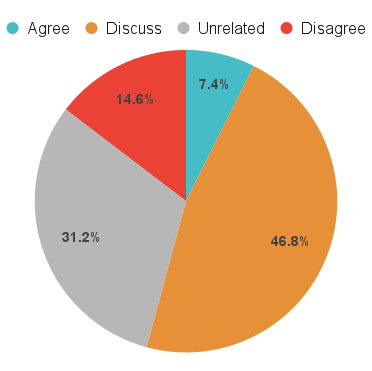
\includegraphics[width=6cm]{statistics/stance/a2c.png} }}%
	\qquad
	\subfloat[\centering Headline to claim ]{{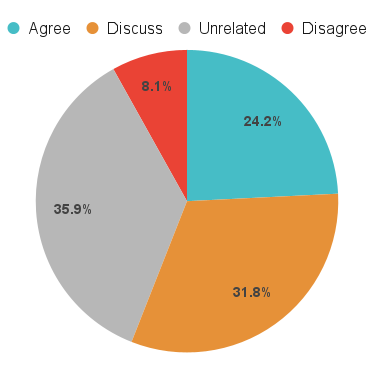
\includegraphics[width=6cm]{statistics/stance/h2c.png} }}%
	\caption{Comparison between Article to claim and Headline to claim labels, samples distribution in \cite{stance_persian} dataset.}%
	\label{fig:datacom}%
\end{figure}

\begin{table}
	\centering
	\caption{Fake news data set statistics}\label{fake-news-dataset}
	\small
	\setlength{\extrarowheight}{5pt}%
	\begin{tabularx} {0.7\textwidth}{ 
			| >{\centering\arraybackslash}X 
			| >{\centering\arraybackslash}X 
			| >{\centering\arraybackslash}X 
			| >{\centering\arraybackslash}X | }
		\hline 
		{\bf Used case}      & {\bf True} & {\bf False} & {\bf Unknown} \\ \hline  \hline
		{Test set}     &      {20}      &      {250}      &  {8} \\ 
		\hline
		{Training set}    &     {91}      &      {1003}       &   {35}\\
		\hline
			{Overall}    &     {111}      &      {1253}       &   {43}\\
		\hline
	\end{tabularx}
	\label{tbl:fakedata}
\end{table}

\begin{figure}%
	\centering
	{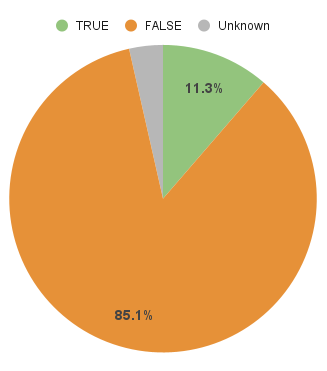
\includegraphics[width=5.5cm]{statistics/stance/fake.png} }
	\caption{Claim veracity label's distribution in \cite{stance_persian} dataset.}%
	\label{fig:fake}%
\end{figure}
  



\section{Tokenizetion}
Tokenization of \textit{Hazm}, \textit{Stanza}, \textit{NLTK}, and \textit{WordPiece} are evaluated against each other manually. Every single difference in each algorithm performance is evaluated\footnote{All different cases during corpus tokenization by those 4 algorithms are gathered in \href{https://docs.google.com/document/d/1SlRBnoyLntLJ5yalWXZ1EqJ0wRj4DyiEMJdewkEkrTM/edit?usp=sharing}{here}}. Only three cases are presented as examples to compare each tokenizer's performance in figure \ref{fig:tekenres}. As we need to remove particular words and patterns from the corpus,  it is important to find a tokenizer that distinguishes all words correctly. Besides, it shouldn't lose information while tokenizing and be as fast as possible. 

In figure \ref{fig:tekenres}, unsuitable tokens are highlighted in blue. There isn't any flawless algorithm. WordPiece is subwords based so there are some UNK tokens and words are wrongly broken. For example figure \ref{fig:tekenres}, part (b) blue highlighted word is broken into two pieces wrongly. Considering connected pronouns individually is the strength of \textit{Stanza} tokenizer. But sometimes the \text{Stanza} wrongly breaks an original word with a wrong assumption that the desired word has a connected pronoun. Figure \ref{fig:tekenres}, part (c) is a sample on wrong separating pronoun and at part (b), pronouns are separated correctly. It can be seen in figure \ref{fig:tekenres} \textit{Hazm}'s performance is highly similar to \textit{NLTK}. The only difference is that in contrast to \textit{NLTK}, Hazm separates numbers and punctuation in the corpus (Figure \ref{fig:tekenres}, part (a)). 

\begin{figure}%
	\centering
	\subfloat[\centering]{{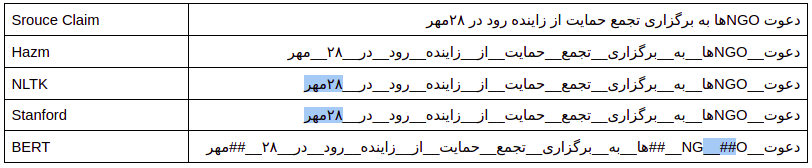
\includegraphics[width=16cm]{statistics/tokenizer/1.png} }}%
	\qquad
	\subfloat[\centering ]{{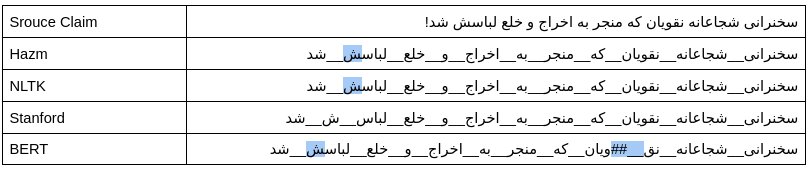
\includegraphics[width=16cm]{statistics/tokenizer/2.png} }}%
	\qquad
	\subfloat[\centering]{{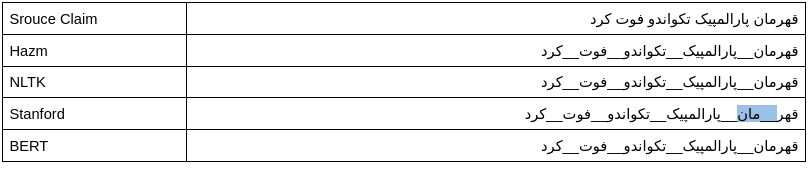
\includegraphics[width=16cm]{statistics/tokenizer/3.png} }}%
	\caption{Comparison performance of \textit{Hazm}, \textit{Stanford}, \textit{NLTK} and \textit{BERT} tokenizers.}%
	\label{fig:tekenres}%
\end{figure}

	Besides, the duration of tokenizing for each tokenizer is compared in figure \ref{fig:tokentime}. While \textit{Hazm} is the fastest words tokenizer among evaluated algorithms, \textit{Stanford} tokenizer lasts significantly longer. According to all pieces of evidence, \textit{Hazm} tokenizer is the best tokenizer for this task.

\begin{figure}%
	\centering
	{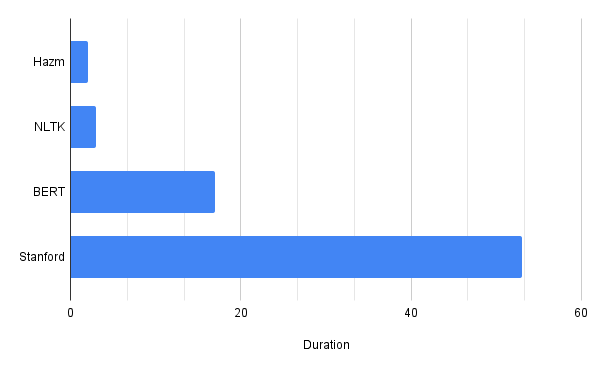
\includegraphics[width=12.5cm]{statistics/tokenizer/duration.png} }
	\caption{Comparison duration of tokenizing algorithm on \cite{stance_persian} dataset.}%
	\label{fig:tokentime}%
\end{figure}

\section{Stop-Words}
After preprocessing tokens, stop-words will be removed from the tokens. Firstly, the same stop-words list which has been used by \cite{stance_persian} was used in the project. After reviewing preprocessed corpus, it was hard to infer the stance from text pieces. So we chose stop-words carefully in a way not to lose refuting or supporting expressions.

Kharazi\footnote{\label{fn:kharazi}github.com/kharazi/persian-stopwords} has classified Persian stop-words into verbal, nonverbal, and short. Verbs carry valuable information in news. Nonverbal stop-word class is a better choice to remove low-value words in this task. Besides, we added and removed some words from Nonverbal list to become suitable for the news context. 


The difference between the performance of these four sets of stop-words in addition to skipping removing stop-words (To have a fair comparison) is illustrated in figure \ref{fig:stopwords}. \cite{stance_persian} contains 1255 words which include wide a range of parts of speech. In contrast, NonVerbal\footnote{Gathered by \href{github.com/kharazi/persian-stopwords}{Kharazi}} stop words set includes 158 words and it doesn't support any verb. In the new version of stop-words, 18 stop words are removed from the Nonverbal set. This set is called \textit{shortened} and 82 new words are added. Finally, the \textit{Extended} version contains 233 words. To evaluate the performance of each stop-words sets, all desired features with Tf-iDF as word representation after removing particular stop words are fed into an SVM (\cite{svc}) model.

It can be inferred from figure \ref{fig:stopwords} that the list of stop-words which is used by \cite{stance_persian} is ignoring valuable data and it is even better not to remove stop-words from the corpus. Nonverbal stop-words achieve higher accuracy on stance detection. Through, whether removing or adding words from Nonverbal (\textit{shortened} version) didn't improve results. Altogether, Nonverbal list of stop-words, performs the best in this task. 
Then all remaining tokens will be concatenated with a space character and considered as prepossessed and clean corpus.

\begin{figure}%
	\centering
	{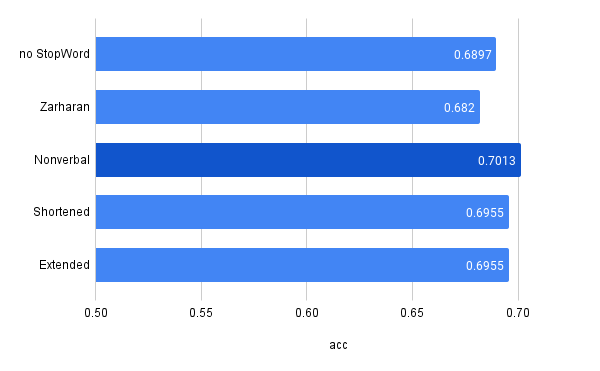
\includegraphics[width=12.5cm]{statistics/AccuracyScore.png} }
	\caption{Comparison accuracy of SVM model with different configuration of stop words.}%
	\label{fig:stopwords}%
\end{figure}

\section{Word Representation}
As a baseline, three different Bag-of-word (\cite{bow}), TF-iDF (\cite{tfidf}), and Word-to-Vector (\cite{word2vec}) algorithms are evaluated against each other. More details are explained in section \ref{lr:wordrep}.

In this project, FastText\footnote{fasttext.cc} Word2Vec model is used with vector lengths equal to 300 which is trained on the Persian Wikipedia website. For both TF-iDF and BoW n-gram range is set from 1 to 2. 

BoW (\cite{bow}), TF-iDF, and Word2Vec (\cite{word2vec}) performances are compared by the SVM machine learning algorithm in the stance detection task. According to figure \ref{fig:wordrep} Tf-iDF performs the best in comparison to BoW and Word2Vec in order to represent words.
\begin{figure}%
	\centering
	{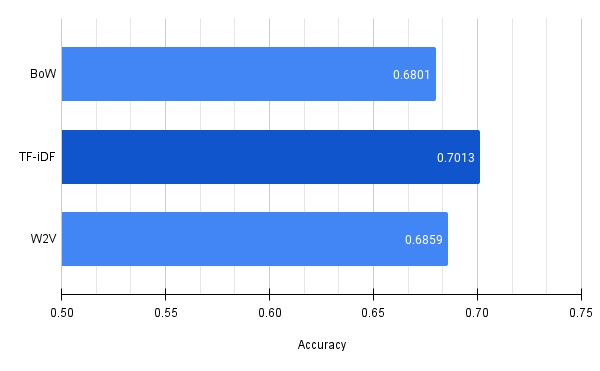
\includegraphics[width=12.5cm]{statistics/WordRep.png} }
	\caption{Comparison SVM model with Bow, TF-iDF and Word2Vec word representaion algorithms.}%
	\label{fig:wordrep}%
\end{figure}

\section{Predictors}
\label{sec:predictors}
Different combinations of calculated predictor are run to find out that which set of predictors performs better. Desired predictors are Similarity, RootDistance, IsQuestion, HasTwoParts and Polarity. In this Section, both SVM (\cite{svc}) and RandomForest (\cite{randomforest}) results are considered in evaluation to have a more accurate analysis. The similarity score is calculated by utilizing \textit{difflib}\footnote{docs.python.org/3/library/difflib.html} python library.


Firstly, both models are trained on the corpus representation by TF-iDF without any other predictor. Then, each predictor is added into TF-iDF vector to evaluate their effectiveness individually, and finally, all features together are fed to models. According to table \ref{tlb:predictors}, Similarity and ImportantWords have the highest positive effect respectively, on both accuracy (\ref{eq:acc}) and f1-score (\ref{eq:f1}). Similarity score has improved accuracy 15 to 17 percent and ImportantWords has improved SVM accuracy by almost 4 percent. Though, predictors such as IsQuestion, HasTwoParts, and Polarity don't have a significant effect on results, using them all together boost total accuracy and f1-score. 

Due to figure \ref{tlb:predictors}, using RootDistance, IsQuestion, and HasTwoParts individually decreases accuracy, so models are also trained with two other variations. Though IsQuestion, HasTwoParts, and polarity don't have a positive effect individually, using them with Similarity, ImportantWrods, and polarity boost accuracy. On the other hand, removing RootDistance from All predictors mode whether has a negligible effect or improves accuracy. 

According to previous comparisons and evaluation inferred from table \ref{tlb:predictors}, the best predictors to use for stance detection task is the combination of Similarity, ImportantWords, IsQuestion, HasTwoParts, and Polarity predictors in addition to TD-iDF as the corpus representer, altogether.

\begin{table}
	\centering
	\caption{Comparison of accuracy score and F1-score with different combinations of predictors for both SVM and Random Forest classifiers.}
	\setlength{\extrarowheight}{5pt}%
	\begin{tabular*}{350pt}{@{\extracolsep{\fill}}| l | l | l | l | l |}
		\hline
		\multicolumn{1}{|c|}{} & \multicolumn{2}{l|}{SVM} & 
		\multicolumn{2}{l|}{RandomForest}  \\ \cline{2-5} 
		
		\multicolumn{1}{|c|}{\multirow{-2}{*}{\begin{tabular}[c]{@{}c@{}}Predictors\\  Model\end{tabular}}}         & Acc.    & F1.    & Acc.    & F1.    \\ \cline{1-1}
		
		\hline \hline
		
		\multicolumn{1}{|c|}{TF-iDF only} & 51.83   & 51.90   & 52.79   & 54.00   \\ \cline{1-1}
		\hline
		+ Similarity      		& 66.85   & 66.71   & 68.78   & 67.88   \\ \cline{1-1}
		\hline
		+ Root Distance   		& 51.25   & 51.50   & 49.71   & 50.52   \\ \cline{1-1}
		\hline
		+ Important Words 		& 56.64   & 56.94   & 52.98   & 52.49   \\ \cline{1-1}
		\hline
		+ Is Question     		& 51.63   & 51.79   & 51.63   & 52.70   \\ \cline{1-1}
		\hline
		+ Has Two Parts   		& 51.83   & 51.90   & 50.28   & 50.87   \\ \cline{1-1}
		\hline
		+ Polarity        		& 52.21   & 52.50   & 52.40   & 53.25   \\ \cline{1-1}
		\hline
		+ All                   & 69.74   & 69.75  & 69.36   & 68.75   \\ \cline{1-1}
		\hline
		+ All - Root Distance   & 69.74   & 69.69   & \textbf{70.71}   & \textbf{70.28}   \\ \hline
		+ Similarity + ImportantWords   & 69.74   & 69.69   & 67.82  & 67.02  \\ \hline
	\end{tabular*}
	\label{tlb:predictors}
\end{table}

\section{Machine Learning}
\label{sec:ml}
In this section, each Gaussian Naive Bayes, SVM, Linear SVC, Random Forest, and Logistic Regression parameters are tuned on stance detection task with respect to chosen predictors in the previous section (\ref{sec:predictors}). In the next step, the performance of models is compared to each other.

\subsection{SVM}
In this project, We adopted SVC model implementation from \textit{scikit-learn}\footnote{scikit-learn.org/stable/modules/generated/sklearn.svm.SVC.html} python library is used in this project. \textit{class\_weight} parameter set to \textit{balanced} to compensate imbalanced data. Three SVM classifier tuned parameters  are Kernel, Regularization parameter (C) and degree of polynomial kernel. Evaluated kernels are RBF, Polynomial and Sigmoid. According to figure \ref{fig:svm}, Sigmoid works weak for this task. Each polynomial kernel behaves differently due value of the regularization parameter. Polynomial with degrees 2 and 3 perform better than 1 and 4. Linear polynomial may be so simple and SVM is not good enough to classify stance with a polynomial with degree 4. RBF, Polynomial degree 3 behave similarly due to the regularization parameter changes. 

The best configuration for SVM classifier is using RBF as the kernel with regularization parameter equal to 2.5 confirming figure \ref{fig:svm}. Learning procedure and details of each model training exist in this project GitHub repository\footnote{Different SVM configuration training details \href{https://github.com/mahsaghn/stance\_detection/tree/main/selected\_outputs/machinelearning/svm}{[here]}.}.

\begin{figure}% 
	\centering
	{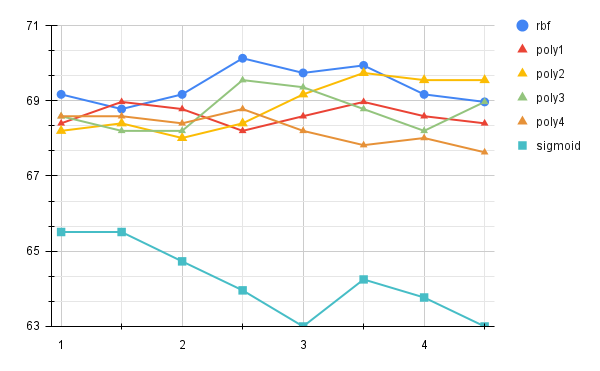
\includegraphics[width=12.5cm]{statistics/svm.png} }
	\caption{Tuning SVM model parameters with TF-iDF representation algorithms}%
	\label{fig:svm}%
\end{figure}

\subsection{Linear SVC}
Linear Support Vector Machine Classifier algorithm, loss function and Regularization parameters are tuned with penalty equals to \textit{l2}. Figure \ref{fig:linearsvm} illustrates comparison between linear svm models with loss functions equal to Hinge or Squared Hinge, and tuned SVM algorithm. Hinge loss function has scored better performance than Squared Hinge. When Squared Hing is used as loss function, as the Regularization parameter increases, accuracy score decrease. Though Regularization parameter don't have significant effect on accuracy score when loss is equal to Hinge. In conclusion, due to figure \ref{fig:linearsvm} Best configuration is for Hinge loss and Regularization parameter equals to 1.0. 
\begin{figure}% 
	\centering
	{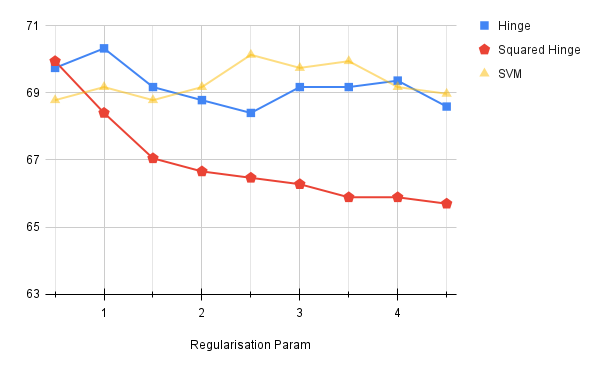
\includegraphics[width=12.5cm]{statistics/linearsvm.png} }
	\caption{Tuning LinearSVC model parameters with TF-iDF representation algorithms.}%
	\label{fig:linearsvm}%
\end{figure}
\subsection{Random Forest}
In this project, implemented Random Forest algorithm from \textit{scikit-learn}\footnote{scikit-learn.org/stable/modules/generated/sklearn.ensemble.RandomForestClassifier.html} python library is used. Three parameters of \textit{max\_features} (Maximum number of features allowed to use for each tree), \textit{estimator} (Number of decision trees), and \textit{criterion} (Algorithm to measure the quality of splits in nodes) are tuned for the desired task.

Figure \ref{fig:randomforest} illustrates the effect of the number of trees in the forest on accuracy among different configuration. The average accuracy score of models increases by adding more trees into the forest. Besides, \textit{gini} algorithm performs better than \textit{entropy} to measure the quality of splits. Also, three different upper bounds are considered for number of features when looking for a split. No boundary, \textit{sqrt} of total features and \textit{log2} of total feature. According to figure \ref{fig:randomforest} don't apply any boundary leads to better accuracy on average. Furthermore, as the boundary gets tighten average performance decreases. 

The best configuration for Random Forest machine learning model in this task is using \textit{gini} algorithm to evaluate splitting quality, not applying any boundary on the number of features and having 125 decision trees in the forest. 
\begin{figure}% 
	\centering
	{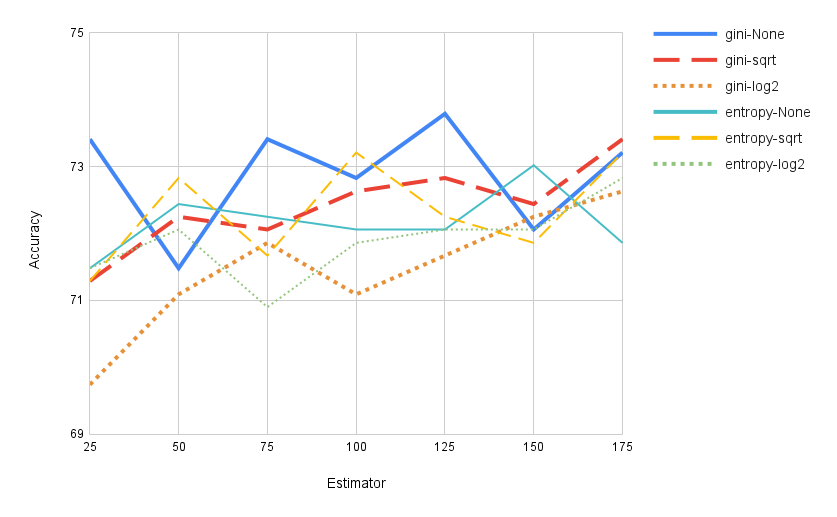
\includegraphics[width=12.5cm]{statistics/randomforest.png} }
	\caption{Random Forest machine learning model different configuration on stance detection task. Type of line presents type of the boundary applied on each model. Solid line, dash line and doted line stands for no boundary, sqrt of total feature and log2 of total feature respectively.}%
	\label{fig:randomforest}%
\end{figure}
\subsection{Logistic Regression}
We also adopted the Logistic Regression algorithm from the \textit{sckiti-learn}\footnote{scikit-learn.org/stable/modules/generated/sklearn.linear\_model.LogisticRegression.html} python library. Many experiments are designed to evaluate behavior of Logistic Regression models. 	 \textit{Elasticnet} (Equation \ref{eq:logisel}) penalty algorithm which is used in penalization procedure, used for \textit{saga} solver and \textit{l2} penalty algorithm is used for \textit{sag}, \textit{lbfgs}, and \textit{newton-cg} solvers. 

\textit{Elasticnet} has a $\rho$ parameter which determines the portion of using $l1$ to $l2$ penalty in \textit{saga} solver. Figure \ref{fig:logistic1} illustrate the effect of $\rho$ values from $0$ to $0.9$ on the accuracy of stance detection. Besides, models with a regression parameter from $0.5$ to $4.5$ are evaluated from the determined $\rho$ range. It can be inferred from figure \ref{fig:logistic1} that $\rho$ parameter doesn't have a significant effect on the accuracy of the model. While regression parameter between $1$ and $2.5$ clearly results in higher accuracy rather than external range. It can be also inferred from figure \ref{fig:logistic2} which illustrates the effect of the regression parameter on stance classification accuracy. Models with different values of $\rho$ behave similarly and best performances happen when regression parameter is between $1$ and $2.5$.  
\begin{figure}% 
	\centering
	{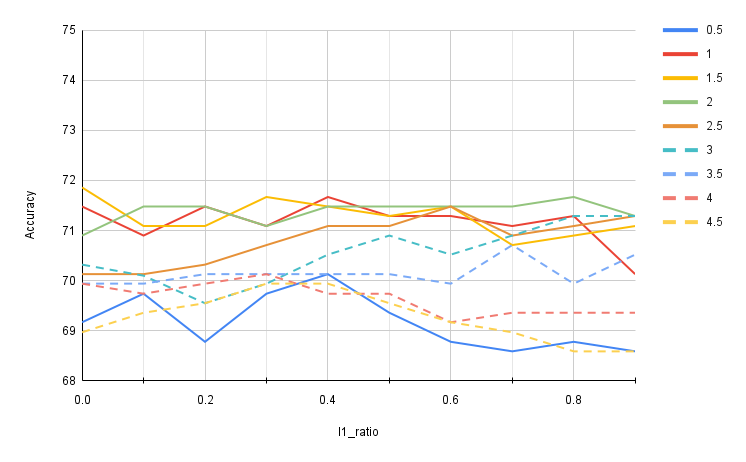
\includegraphics[width=12.5cm]{statistics/logistic_elastic1.png} }
	\caption{Effect of $\rho$ parameter of \textit{elasticnet} penalty on stance detection task.}%
	\label{fig:logistic1}%
\end{figure}
\begin{figure}% 
	\centering
	{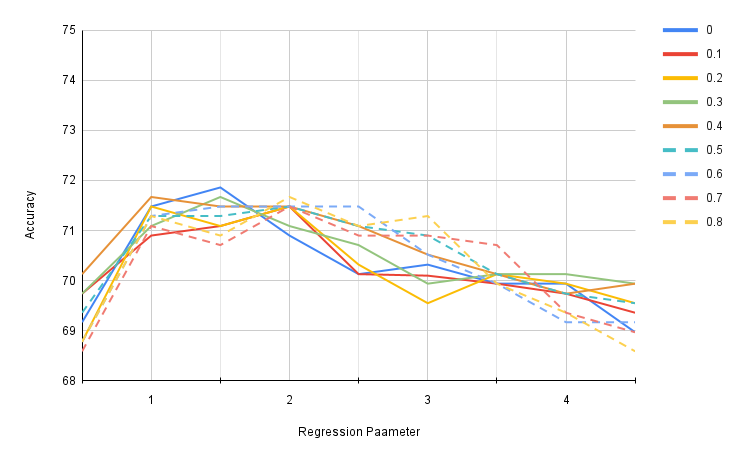
\includegraphics[width=12.5cm]{statistics/logistic_elastic2.png} }
	\caption{Effect of regression parameter of \textit{elasticnet} penalty on stance detection task.}%
	\label{fig:logistic2}%
\end{figure}

Another variant of Logistic Regression setup is to use $l2$ penalty with desired solver algorithms. Figure \ref{fig:logistic3} compares best \textit{saga} solver with \textit{sag}, \textit{lbfgs}, and \textit{newton-cg}. The Logistic Regression with \textit{lbfgs} solver and regression parameter equals 1.5 has recorded the highest accuracy. 
\begin{figure}% 
	\centering
	{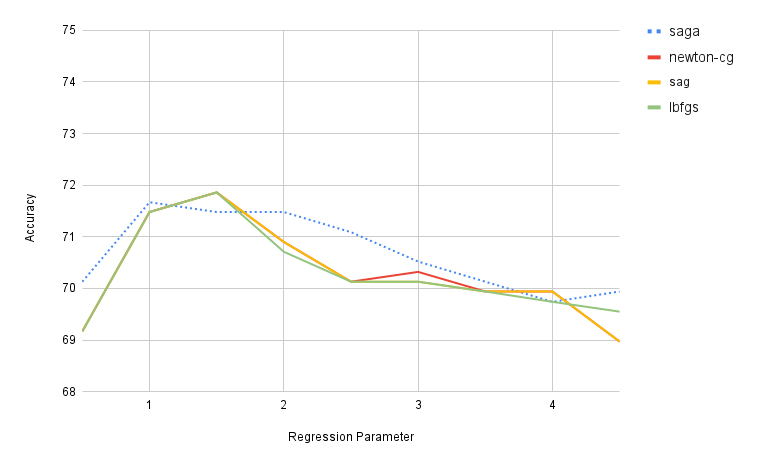
\includegraphics[width=12.5cm]{statistics/logistic1.png} }
	\caption{Comprasion of Logistic Regression machine learning models.}%
	\label{fig:logistic3}%
\end{figure}

\subsection{Comparison}
In previous sections parameters of each SVM, LinearSVC, Random Forest, and Logistic Regression models are tuned. In this section models with desired parameters have run 5 times each to have more reliable results and comparison. Average accuracy and highest accuracy recorded in tuning phase, compared in figure \ref{fig:all}. The highest achievable accuracy with machine learning models to classify the stance of a claim towards the headline of a news article is 74.01\%.
\begin{figure}% 
	\centering
	{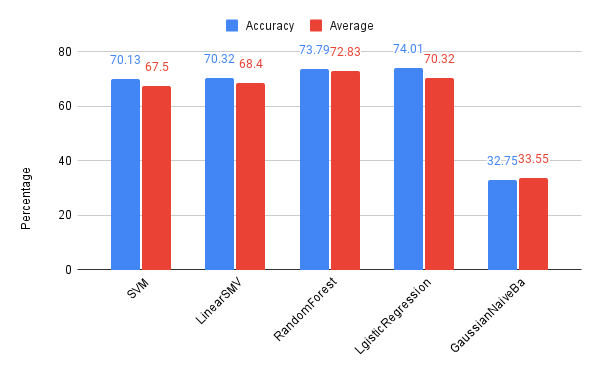
\includegraphics[width=12.5cm]{statistics/machinlearning.png} }
	\caption{Comparison SVM model between Bow, TF-iDF and Word2Vec word representation algorithms.}%
	\label{fig:all}%
\end{figure}
\section{Dataset Balancing}
As mentioned in section \nameref{sec:dataset}, Figure \ref{fig:datacom}, the number of samples in dataset classes was imbalanced. So oversampling should be performed in classes except for the majority class.
In \cite{stance_persian} minority class forms only 7.4\% of data (Figure \ref{fig:datacom}).
 All oversampling methods are evaluated against each other in this project and utilized from the oversampling package of \textit{imblearn} \footnote{imbalanced-learn.org/stable/references/over\_sampling.html} python library. 

\begin{figure}%
	\centering
	\subfloat[\centering Artcile to Claim]{{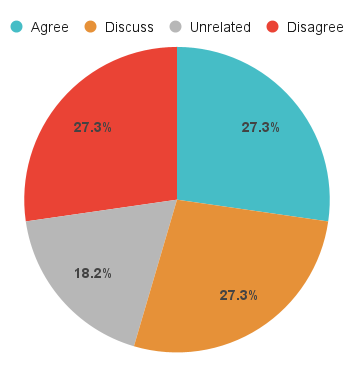
\includegraphics[width=6cm]{statistics/stance/a2c_b1.png} }}%
	\qquad
	\subfloat[\centering Headline to claim ]{{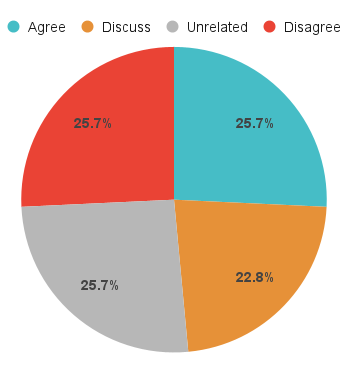
\includegraphics[width=6cm]{statistics/stance/h2c_b1.png} }}%
	\caption{Comparison between article-to-claim and headline-to-claim labels, samples distribution in \cite{stance_persian} dataset, after extending by \cite{parsfever} .}%
	\label{fig:datab1}%
\end{figure}



Firstly, ADASYN, SMOTE, SVMSMOTE, BorderLineSmote, and RandomOverSampler oversampling methods are applied on the \cite{stance_persian} dataset. In ADASYN algorithm, the number of nearest neighbors to generate a new sample is set to 9\footnote{imbalanced-learn.org/stable/references/generated/imblearn.over\_sampling.ADASYN.html}. Each method is evaluated against five desired machine learning models. Red series in figure \ref{fig:balanc} stands for the accuracy of models, associated with the \cite{stance_persian} dataset. LinearSVC, LogisticRegresion, and GaussianNaibeBayes are not compatible with any oversampling method. Though, ADASYN oversampling method has increased these two model accuracy $5$ percent on average.


In the second step, the dataset is extended by the ParsFever (\cite{parsfever}) dataset. Though the number of samples is increased accuracy is obviously decreased, but the GaussianNB model. This may happen that data sources from each dataset are totally different and headlines in ParsFever are much longer than the \cite{stance_persian} dataset.
\begin{figure}% 
	\centering
	{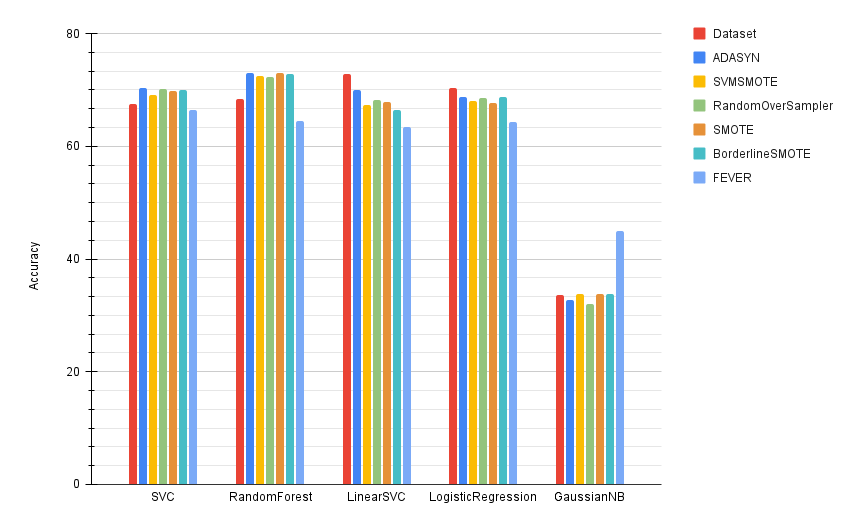
\includegraphics[width=14.5cm]{statistics/balancing.png} }
	\caption{Comparison SVM model with Bow, TF-iDF and Word2Vec word representation algorithms.}%
	\label{fig:balanc}%
\end{figure}

\section{Deep Learning}

\label{sec:dl}
A Pre-trained BERT-based model is used at the top of the model, then two Dense layers and finally a Dense including 4 neurons to classify stance is considered for the end-to-end system. The input of our deep learning models is \textit{input ids}, \textit{token type ids}, and \textit{attention mask}.
BERT (\cite{bert}), ParsBERT \cite{parsbert}, and ALBERT (\cite{albert}) models are substitute with Pretrained ML model in figure \ref{fig:dlschm}. Each epoch lasts about 26 seconds in the training procedure. Figure \ref{fig:deep} illustrates the model training procedure. In comparison to machine learning models, the deep learning model has boosted the accuracy of headline-to-claim stance detection by 10 percent. 

The BERT-based model has been learned for 20 epochs. Validation loss has been stated to increase since epoch 11 and validation accuracy hasn't changed considerably then. Best validation accuracy has converged on $80.92\%$ on the headline-to-claim dataset. 

The ParsBert-based model has been learned for 20 epochs. Best validation accuracy has converged on $81.11\%$ on the headline-to-claim dataset. In comparison to the machine learning algorithm, deep learning algorithm has enhanced about $10\%$ accuracy. Besides, the loss score has converged on a lower score than BERT-based model.

Though, the best recorded ALBERT language model on 20 epochs is at most $70.52\%$ on accuracy score. Figure \ref{fig:deep}, parts (e) and (f) is illustrated the training procedure.

Among these three alternatives of the BERT algorithm, PasrBERT based model has recorded the best accuracy score with $85.48\%$ accuracy on stance prediction.  
\begin{figure}%
	\centering
	\subfloat[\centering]{{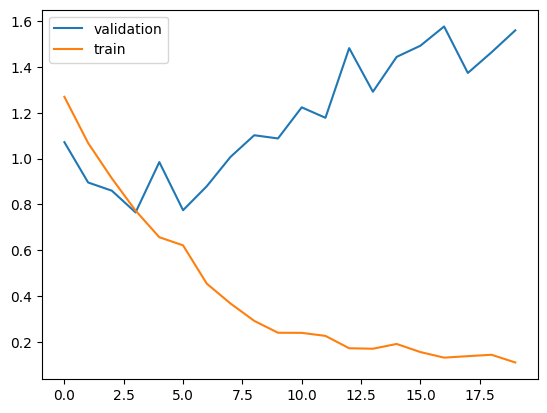
\includegraphics[width=6cm]{statistics/deep/bert_loss.png} }}%
	\qquad
	\subfloat[\centering]{{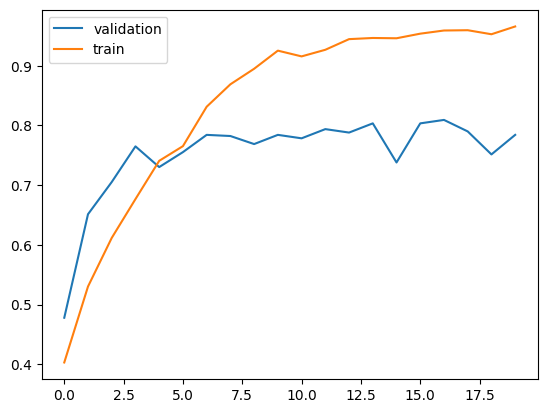
\includegraphics[width=6cm]{statistics/deep/bert_acc.png} }}%
	\qquad
	\subfloat[\centering]{{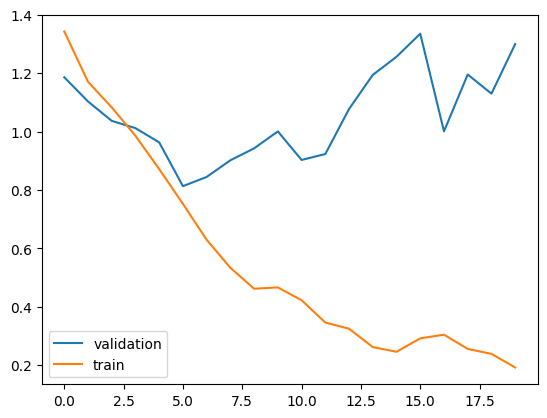
\includegraphics[width=6cm]{statistics/deep/parsbert_loss.png} }}%
	\qquad
	\subfloat[\centering]{{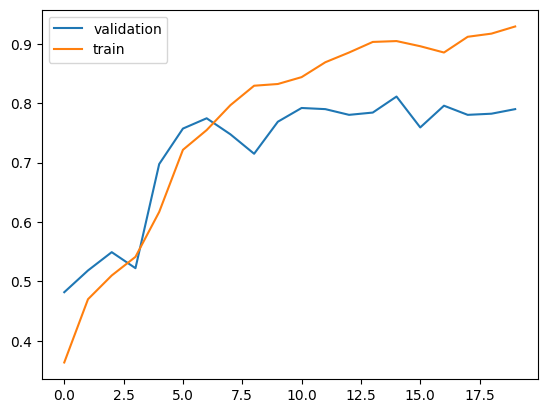
\includegraphics[width=6cm]{statistics/deep/parsbert_acc.png} }}%
	\qquad
	\subfloat[\centering]{{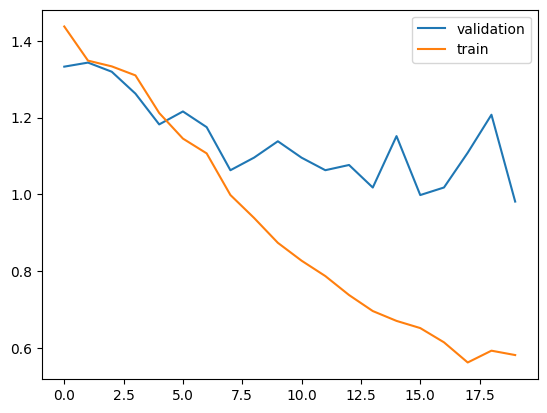
\includegraphics[width=6cm]{statistics/deep/albert_loss.png} }}%
	\qquad
	\subfloat[\centering]{{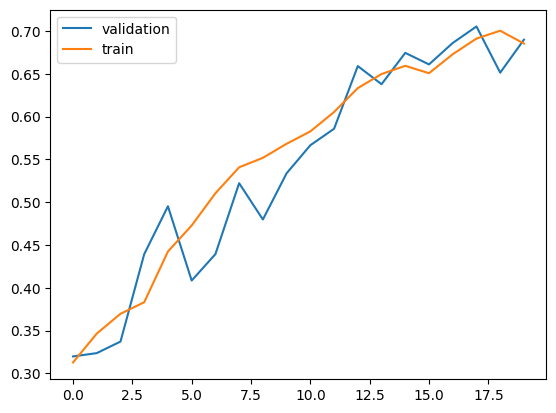
\includegraphics[width=6cm]{statistics/deep/albert_acc.png} }}%
	
	
	\caption{Deep learning procedure on the headline-to-claim stance detection task. Left figures illustrate loss score and right figures illustrate accuracy score of train and test data during the training procedure. (a, b) Pre-trained language model based on Google's BERT (\cite{parsbert}) on Persian corpus (c, d) Pre-trained monolingual language model based on ParsBERT (\cite{parsbert}) on Persian corpus. (e, f) Pre-trained language model based on ALBERT (\cite{albert}) on Persian corpus}%
	\label{fig:deep}%
\end{figure}

\begin{table*}[t]
	\centering
	\small
	\caption{Comparison of headline-to-claim stance detection models.}
	\def\arraystretch{1.3}%
	\setlength{\extrarowheight}{5pt}%
	\begin{tabular}{|c|c|c|c|c|}
		\hline{Model} & {Precision} & {Recall} & {F1} & {Accuracy}\\
		\hline \hline
		{SVM+ADASYN} & {69.63} & {69.15} & {69.38} & {70.32}\\
		\hline
		{RandomForest+ADASYN} & {71.24} & {69.14} & {70.17} & {73.02}\\
		\hline
		{BERT} & {81.65} & {80.69} & {81.16} & {80.92}\\
		\hline
		{ParsBERT} & {84.67} & {79.42} & {81.96} & {81.11}\\
		\hline
		{ALBERT} & {75.75} & {64.09} & {69.43} & {70.52}\\
		\hline
		{ParsBERT+ADASYN} & {84.96} & {85.64} & {85.29} & {\textbf{85.48}}\\
		\hline
	\end{tabular}
	\label{tbl:allstance}
\end{table*}


\section{Article to Claim}

Best stance detection models on both machine learning and deep learning models are evaluated on article-to-claim task. The length of 400 characters is considered for the maximum length of article content. Table \ref{tbl:allstance} show those models performance on both headline-to-claim and article-to-claim task. Using ADASYN oversampler and ParsBERT as the pre-trained language leads to our best results on both headline-to-claim and article-to-claim models. We achieved 80.62\% accuracy score on the article-to-claim task. Out experiments on article-to-claim achieved a lower score than the headline-to-claim task because inferring from longer text is a harder task for the model.  

\begin{table*}[t]
	\centering
	\small
	\caption{Comparison between article-to-claim machine learning and deep learning models.}
	\def\arraystretch{1.3}%
	\setlength{\extrarowheight}{5pt}%
	\begin{tabular}{|c|c|c|c|c|}
		\hline
		{} & \multicolumn{2}{c|}{Headline to claim} &  \multicolumn{2}{c|}{Article to claim}\\
		\hline 
		{Model} & {F1} & {Accuracy} & {F1} & {Accuracy}\\
		\hline	\hline
		{SVM+ADASYN} & {69.38} & {70.32} & {65.18} & {64.49}\\
		\hline
		{ParsBERT} & {81.96} & {81.11} & {78.00} & {78.32}\\
		\hline
		{ParsBERT+ADASYN} & {85.29} & \textbf{{85.48}} & {80.29} & \textbf{{80.62}}\\
		\hline
	\end{tabular}
	\label{tbl:a2c}
\end{table*}

\section{Fake News}
The best BERT-based model for headline-to-claim and article-to-claims are considered for this part. These model prediction base on 4 news articles are concatenated with features which are described in section \ref{sec:fakenews}. Then the overall vector is feed to a three-layer MLP model as the classifier. ADASYN oversampling method is also used to deal with imbalanced classes. Figure \ref{fig:fakenews} illustrates the training procedure before oversampling and after oversampling the dataset. After oversampling, the trained model accuracy has converged to 99\%, while before oversampling model stops at $90.41\%$. According to figure \ref{fig:fakenews}, after adding oversampled samples, at first iterations, it is harder for the model to decrease the loss score on the train set and loss score convergent takes a longer time. Though after balancing the dataset (Figure \ref{fig:fakenews}, part (a)), the value of loss score has converged 0.2 lower than the original dataset (Figure \ref{fig:fakenews}, part (c)).

\begin{figure}%
	\centering
	\subfloat[\centering]{{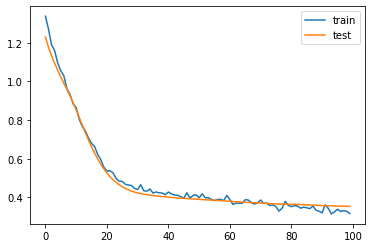
\includegraphics[width=6cm]{statistics/fakenews/dataset/loss.png} }}%
	\qquad
	\subfloat[\centering]{{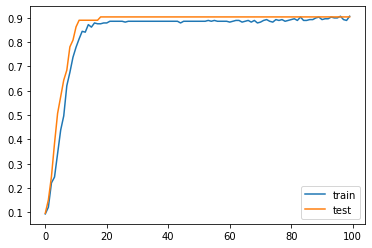
\includegraphics[width=6cm]{statistics/fakenews/dataset/acc.png} }}
	\qquad
	\subfloat[\centering]{{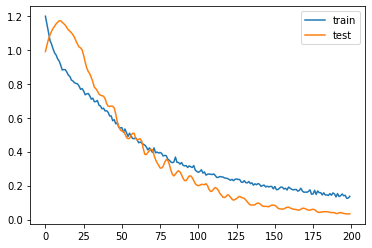
\includegraphics[width=6cm]{statistics/fakenews/oversampled/loss.png} }}%
	\qquad
	\subfloat[\centering]{{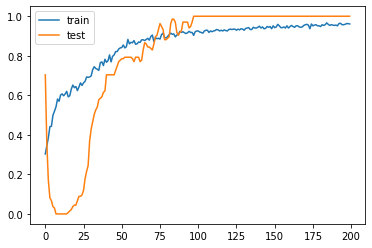
\includegraphics[width=6cm]{statistics/fakenews/oversampled/acc.png}}}
	\caption{Left figures illustrate loss score and right figures illustrate accuracy score of train and test data during training procedure for each iteration. 
		(a, b) Training procedure on fake news detection model trained on the \cite{stance_persian} dataset.
		(c, d) Training procedure on fake news detection model trained on oversampled \cite{stance_persian} dataset by ADASYN (\cite{adasyn}) algorithm.}%
	\label{fig:fakenews}%
\end{figure}

\chapter{Conclusion}
Machine learning models are evaluated on Persian stance detection task as baseline. Multiple predictors are extracted and different combination of them are applied on machine learning models to find out the most effective predictor combination. Due imbalanced samples distribution in the \cite{stance_persian} dataset, extending the dataset by ParsBERT dataset (\cite{parsbert}) and oversampling methods are discussed and compared to each other.

In the Persian stance detection task, using deep language models boosts performance noticeably. BERT and ParsBERT as it's alternative have high ability to make inference from a given content so they can represent current content sufficiently and test accuracy in the model based on ParsBERT language model is equal to 85.48\%. As the result,  BERT language models predict stance detection 10\% higher than machine learning algorithm on average. In contrast, requires time consuming feature engineering and parameter tuning and they can't achieve high accuracy on language inference tasks. For both machine learning and deep learning models performance decrease on article-to-claim task. Despite of this issue, machine learning algorithm have achieve even higher than 70\% accuracy score on headline-to-claim task. The black-box nature of machine learning algorithms means that nobody really knows why an AI lie detection system works as it does, nor what it is actually doing (\cite{book_fake}). 

The best pretrained stance detection model on headline-to-claim and article-to-claim are separately utilized in fake news detection. We have achieve 99\% accuracy score on the \cite{stance_persian} dataset. Though, number of samples in the dataset gathered by \cite{stance_persian} contains 1624 samples. Increasing number of samples help model to improves model generalization.

Adding attention layers to the classifier have improve results in current researches. Fox instance, \cite{book_disinformation} alleged that using attention layers in the model have make a great contribution on accuracy scores. Utilizing such models can also make increase on the ability of these models to go beyond the current state in such low-resource settings. Besides, increasing number of samples in the \cite{stance_persian} dataset toward achieving balanced dataset can help the model to distinguish each class precisely. 
 
 
 

\renewcommand{\bibname}{References}
\bibliography{main.bib}	
\bibliographystyle{acl_natbib}

% Optionally: add appendices
\newpage
\newcommand{\beginsupplement}{%
    \setcounter{chapter}{0}
    \renewcommand{\thechapter}{\Alph{chapter}}%
 }

\beginsupplement
\begin{comment}
	\chapter{Appendix One}
	\section{Appendix section 1}
	\begin{table}[]
	\centering
	\begin{tabular}{c|c}
	&  \\
	& 
	\end{tabular}
	\caption{Table in the Appendix}
	\label{tab:my_label}
	\end{table}	
\end{comment}
\newpage 

\ % The empty page
\newpage 



\vspace*{3cm}
{
\centering

\includegraphics[width=4cm]{iust.jpeg}
\\
\bigbreak
\centerline {\textbf{Iran University of Science and Technology}}
\bigbreak
\large\centerline {\textbf{Computer Engineering Department}}
}

\end{document}

% you're all done, congrats!